\subsection{Superficial elements}

In this section, let q denote an ideal of A contained in the radical of A, and let M be a nonzero finitely generated A-module such that M/qM has finite length.

PROPOSITION 8. --- Let \(\delta > 0\) be an integer, \(x\) an element of \(\mathfrak{q}^{\delta}\) , \(\xi\) its class in \(\mathrm{gr}_{\delta}(\mathbf{A}) = \mathfrak{q}^{\delta}/\mathfrak{q}^{\delta+1}\) , and \(\varphi\) denote multiplication by \(\xi\) in the \(\mathrm{gr}(\mathbf{A})\) -module \(\mathrm{gr}(\mathbf{M})\) .

\begin{enumerate}
\def\labelenumi{\alph{enumi})}
\item
  The dimension of the A-module M/xM is equal to \(\dim_{\mathbf{A}}(\mathbf{M})\) or to \(\dim_{\mathbf{A}}(\mathbf{M}) - 1\) . In the second case, we have \(e_{\mathfrak{q}}(\mathbf{M}/x\mathbf{M}) \geqslant \delta e_{\mathfrak{q}}(\mathbf{M})\) .
\item
  Suppose that we have \(\dim_{\mathbf{A}}(\mathbf{M}) \geqslant 1\) and that the kernel of \(\varphi\) is of finite length over A/q. Then we have \(\dim_{\mathbf{A}}(\mathbf{M}/x\mathbf{M}) = \dim_{\mathbf{A}}(\mathbf{M}) - 1\) . Moreover:
\end{enumerate}

\begin{enumerate}
\def\labelenumi{(\roman{enumi})}
\item
  If \(\dim_{\mathbf{A}}(\mathbf{M}) > 1\) , one has \(e_{\mathfrak{q}}(\mathbf{M} / x\mathbf{M}) = \delta e_{\mathfrak{q}}(\mathbf{M})\) .
\item
  If \(\dim_{\mathbf{A}}(\mathbf{M}) = 1\) , one has, for every integer \(n \geqslant 0\)
\end{enumerate}

\[
n \delta e _ {\mathfrak {q}} (\mathrm{M}) \leqslant \operatorname{long} _ {\mathrm{A}} (\mathrm{M} / x ^ {n} \mathrm{M}) \leqslant n \delta e _ {\mathfrak {q}} (\mathrm{M}) + \operatorname{long} _ {\mathrm{A} / \mathfrak {q}} (\operatorname{Ker} \varphi^ {n}),
\]

where \(\varphi^n\) is the \(n\) -th iterate of the endomorphism \(\varphi\) , and

\[
\delta e _ {\mathfrak {q}} (\mathbf {M}) = e _ {x \mathbf {A}} (\mathbf {M}) \leqslant \operatorname{long} _ {\mathbf {A}} (\mathbf {M} / x \mathbf {M}).
\]

Set \(\mathbf{M}'' = \mathbf{M} / x\mathbf{M}\) ; consider the Hilbert-Samuel series \(\mathbf{H}_{\mathbf{M}} = \mathbf{H}_{\mathbf{M},\mathfrak{q}}\) and \(\mathbf{H}_{\mathbf{M}''} = \mathbf{H}_{\mathbf{M}'',\mathfrak{q}}\) as well as the Poincaré series \(\mathbf{P}(\mathbf{T}) = \sum_{n\geqslant 0}\mathrm{long}_{\mathbf{A} / \mathfrak{q}}(\mathrm{Ker}\varphi_n)\mathbf{T}^n\) . By § 4, no. 3, th. 2 and no. 4, remark 2, we have

\[
\mathrm{H} _ {\mathbf {M}} (\mathrm{T}) = (1 - \mathrm{T}) ^ {- d} \mathrm{R} _ {\mathbf {M}} (\mathrm{T}), \quad \mathrm{H} _ {\mathbf {M} ^ {\prime \prime}} (\mathrm{T}) = (1 - \mathrm{T}) ^ {- d ^ {\prime \prime}} \mathrm{R} _ {\mathbf {M} ^ {\prime \prime}} (\mathrm{T}),
\]

with \(d = \dim_{\mathbf{A}}(\mathbf{M})\) , \(d'' = \dim_{\mathbf{A}}(\mathbf{M}'')\) , \(\mathbf{R}_{\mathbf{M}}\) and \(\mathbf{R}_{\mathbf{M}''}\) in \(\mathbf{Z}[T]\) , \(\mathbf{R}_{\mathbf{M}}(1) = e_{\mathfrak{q}}(\mathbf{M})\) , \(\mathbf{R}_{\mathbf{M}''}(1) = e_{\mathfrak{q}}(\mathbf{M}'')\) . By Lemma 6 of § 4, no. 5, we have in \(\mathbf{Z}((T))\) the inequalities

\[
\left(1 - \mathrm{T} ^ {\delta}\right) \mathrm{H} _ {\mathbf {M}} ^ {(1)} \leqslant \mathrm{H} _ {\mathbf {M} ^ {\prime \prime}} ^ {(1)} \leqslant \left(1 - \mathrm{T} ^ {\delta}\right) \mathrm{H} _ {\mathbf {M}} ^ {(1)} + \mathrm{T} ^ {\delta} \mathrm{P} ^ {(1)}.
\]

Setting \(\mathrm{R}(\mathrm{T}) = (1 - \mathrm{T}^{\delta}) / (1 - \mathrm{T}) = 1 + \mathrm{T} + \cdots + \mathrm{T}^{\delta-1},\) this is also written

\[
\begin{array}{r l} (1) & (1 - \mathrm{T}) ^ {- d} \mathrm{R(T)} \mathrm {R_ {M} (T)} \leqslant (1 - \mathrm{T}) ^ {- d ^ {\prime \prime} - 1} \mathrm {R_ {M^ {\prime\prime}} (T)} \leqslant \\ & \leqslant (1 - \mathrm{T}) ^ {- d} \mathrm{R(T)} \mathrm {R_ {M} (T)} + (1 - \mathrm{T}) ^ {- 1} \symrm {T^ {\delta} P(T)}. \end{array}
\]

By Lemma 2 of § 4, no. 1, the first inequality (1) implies either \(d'' \geqslant d\) , or \(d'' = d - 1\) and R(1) R \(_{M}\) (1) \(\leqslant\) R \(_{M''}\) (1), that is, \(\delta e_{\mathfrak{q}}(\mathbf{M}) \leqslant e_{\mathfrak{q}}(\mathbf{M}'')\) . This proves \(a\) ), since \(d'' \leqslant d\) .

Under the hypothesis of \(b\) ), we have \(\mathbf{P}(\mathbf{T}) \in \mathbf{Z}[\mathbf{T}]\) and \(\mathbf{P}(1) = \text{long}_{\mathbf{A}}(\text{Ker } \varphi)\) . The second inequality (1) is written

\[
(1 - \mathrm{T}) ^ {- d ^ {\prime \prime} - 1} \mathrm{R} _ {\mathrm{M} ^ {\prime \prime}} (\mathrm{T}) \leqslant (1 - \mathrm{T}) ^ {- d} \left(\mathrm{R} (\mathrm{T}) \mathrm{R} _ {\mathrm{M}} (\mathrm{T}) + \mathrm{T} ^ {\delta} (1 - \mathrm{T}) ^ {d - 1} \mathrm{P} (\mathrm{T})\right).
\]

Suppose we have \(d > 1\) ; then lemma 2 of § 4, no. 1 implies \(d'' + 1 \leqslant d\) , whence \(d'' = d - 1\) according to part \(a\) ) of the proof; we then have

\[
\mathrm{R} _ {\mathbf {M} ^ {\prime \prime}} (1) \leqslant \mathrm{R} (1)\cdot \mathrm{R} _ {\mathbf {M}} (1)
\]

(loc. cit.), whence (i).

Suppose now \(d=1\) . By loc. cit., we have \(d''=0\) and

\[
\mathrm{R} _ {\mathbf {M} ^ {\prime \prime}} (1) \leqslant \mathrm{R} (1)\cdot \mathrm{R} _ {\mathbf {M}} (1) + \mathrm{P} (1).
\]

Consequently, \(\mathbf{M}''\) is of finite length equal to \(e_{\mathfrak{q}}(\mathbf{M}^{\prime \prime}) = \mathbf{R}_{\mathbf{M}''}(1)\) and one obtains

\[
\delta e _ {\mathfrak {q}} (\mathrm{M}) \leqslant \operatorname{long} _ {\mathrm{A}} (\mathrm{M} / x \mathrm{M}) \leqslant \delta e _ {\mathfrak {q}} (\mathrm{M}) + \operatorname{long} _ {\mathrm{A}} (\operatorname{Ker} \varphi).\tag{2}
\]

Let \(n \geqslant 1\) be an integer. Replace \(x\) by \(x^n\) in (2); we therefore have

\[
n \delta e _ {\mathfrak{q}} (\mathbf {M}) \leqslant \operatorname{long} _ {\mathbf {A}} (\mathbf {M} / x ^ {n} \mathbf {M}) \leqslant n \delta e _ {\mathfrak{q}} (\mathbf {M}) + \operatorname{long} _ {\mathbf {A}} (\operatorname{Ker} \varphi^ {n}).\tag{3}
\]

It is immediate that the submodules Ker \(\varphi^{n}\) of the noetherian gr(A)-module gr(M) form an increasing sequence, hence stationary, and that each of them is of finite length over A/q. Dividing by \(n \geqslant 1\) in inequality (3) and letting \(n\) tend to \(+\infty\) , one finds \(e_{xA}(M) = \delta e_{\mathfrak{q}}(\mathbf{M})\) by definition of \(e_{xA}(M)\) .

Lemma 3. — Let R be a graded noetherian ring with degrees ≥ 0, E a finitely generated graded R-module such that \(E_{n}\) is a \(R_{0}\) -module of finite length for every \(n \in Z\). The following conditions are equivalent:

\begin{enumerate}
\def\labelenumi{(\roman{enumi})}
\item
  E is an R-module of finite length;
\item
  there exists an integer \(n_0\) such that \(\mathrm{E}_n = 0\) for \(n \geqslant n_0\) ;
\item
  every prime ideal of \(\mathbf{R}\) associated with \(\mathbf{E}\) contains \(\mathbf{R}_{+} = \bigoplus_{n\geqslant 1}\mathbf{R}_{n}\) .
\item
  \((i) \Leftrightarrow (ii)\): this is clear.
\item
  \((iii) \Rightarrow (i)\): let \(p\) be a prime ideal associated with E. If (iii) is satisfied, we have \(p = p_0 + R_+\) where \(p_0\) is a prime ideal of \(R_0\) and the R-module \(R/p\) is isomorphic to \(R_0/p_0\) . By IV, § 3, n° 1, corollary of prop. 1, the \(R_0\) -module \(R_0/p_0\) is isomorphic to a submodule of one of the \(E_k\) , hence is of finite length. Consequently, R/p is of finite length. By IV, § 2, n° 5, prop. 7, p is therefore maximal. Since p was arbitrary, the R-module E is of finite length (loc. cit.).
\item
  \((i) \Rightarrow (iii)\): let \(p\) be a prime ideal associated with E. Then \(p\) is graded (IV, § 3, no. 1, prop. 1) and maximal (IV, § 2, no. 5, prop. 7), hence contains \(R_{+}\) (§ 6, no. 2, lemma 1).
\end{enumerate}

PROPOSITION 9. --- Let us denote by \(\mathfrak{p}_1, \ldots, \mathfrak{p}_r\) those of the prime ideals of the graded ring \(\mathrm{gr}(\mathrm{A}) = \bigoplus_{n} (\mathfrak{q}^n / \mathfrak{q}^{n+1})\) which are associated with the graded module \(\mathrm{gr}(\mathrm{M}) = \bigoplus_{n} (\mathfrak{q}^n \mathrm{M} / \mathfrak{q}^{n+1} \mathrm{M})\) and do not contain \(\mathrm{gr}_1(\mathrm{A}) = \mathfrak{q} / \mathfrak{q}^2\) . Let \(\delta\) be an integer \(>0\) , \(\xi\) an element of \(\mathrm{gr}_{\delta}(\mathrm{A})\) , and \(\varphi : \mathrm{gr}(\mathrm{M}) \to \mathrm{gr}(\mathrm{M})\) the homothety of ratio \(\xi\) in \(\mathrm{gr}(\mathrm{M})\) . The map \(\varphi_n\) is injective for all \(n\) large enough if and only if \(\xi^n\) does not belong to any of the \(\mathfrak{p}_i\) .

Indeed, the associated prime ideals of the gr(A)-module Ker φ are those among the associated prime ideals of gr(M) that contain ξ (IV, § 1, no. 1, def. 1). By Lemma 3, (Ker φ) \(_n\) is zero for \(n\) large enough, if and only if these ideals all contain \(\mathrm{gr}_{+}(\mathrm{A})\) (or equivalently, \(\mathrm{gr}_{1}(\mathrm{A})\)), hence the proposition.

DEFINITION 2. --- Let A be a Noetherian ring, q an ideal of A contained in the radical of A, and M a finitely generated A-module such that M/qM has finite length. An element x of A is said to be superficial for M relative to q if it belongs to q and if, for all sufficiently large n, the map \(\mathfrak{q}^{n}\mathbf{M}/\mathfrak{q}^{n+1}\mathbf{M} \to \mathfrak{q}^{n+1}\mathbf{M}/\mathfrak{q}^{n+2}\mathbf{M}\) induced by multiplication by x is injective.

Remarks. --- 1) Let δ be an integer \textgreater{} 0. One sometimes says that an element x of A is superficial of order δ for M relative to q if \(x \in \mathfrak{q}^{\delta}\) , and if, for all sufficiently large n, the map \(\mathfrak{q}^{n}\mathbf{M}/\mathfrak{q}^{n+1}\mathbf{M} \to \mathfrak{q}^{n+\delta}\mathbf{M}/\mathfrak{q}^{n+\delta+1}\mathbf{M}\) induced by multiplication by x is injective. With this terminology, the superficial elements in the sense of def. 2 are the superficial elements of order 1.

\begin{enumerate}
\def\labelenumi{\arabic{enumi})}
\setcounter{enumi}{1}
\item
  With the notations of prop. 9, \(x\) is superficial of order \(\delta\) if and only if its class \(\xi\) in \(\mathrm{gr}_{\delta}(\mathbf{A})\) does not belong to any of the \(\mathfrak{p}_i\) .
\item
  By III, § 1, no. 4, Prop. 8, there exists a homogeneous element of \(\mathrm{gr}(\mathrm{A})\) of degree \(>0\) which does not belong to any of the \(\mathfrak{p}_i\) . Consequently, there exists an integer \(\delta > 0\) and a superficial element of order \(\delta\) for M.
\item
  Suppose A is local with residue field \(k\) , and consider the canonical surjective map \(\lambda: \mathfrak{q} \to \mathfrak{q} \otimes_{\mathbf{A}} k\) . It is the composite of the canonical maps \(\mathfrak{q} \to \mathfrak{q}/\mathfrak{q}^2\) and \(\overline{\lambda}: \mathfrak{q}/\mathfrak{q}^2 \to \mathfrak{q} \otimes_{\mathbf{A}} k\) . By Nakayama's lemma, each of the vector subspaces \(V_i = \overline{\lambda}(\mathfrak{p}_i \cap (\mathfrak{q}/\mathfrak{q}^2))\) of \(\mathfrak{q} \otimes_{\mathbf{A}} k\) is distinct from \(\mathfrak{q} \otimes_{\mathbf{A}} k\) ; if \(\alpha \in \mathfrak{q} \otimes_{\mathbf{A}} k\) belongs to none of the \(V_i\) , then \(\lambda^{-1}(\alpha)\) is formed of superficial elements for M (prop. 9). If \(k\) is infinite, the union of the \(V_i\) is distinct from \(\mathfrak{q} \otimes_{\mathbf{A}} k\) and hence there exist superficial elements for M.
\end{enumerate}

THEOREM 1. --- Let A be a Noetherian ring, q an ideal of A contained in the radical of A, and M a finitely generated A-module such that M/qM has finite length. Let \(x_{1}, \ldots, x_{m}\) be a finite sequence of elements of q. Put \(x = Ax_{1} + \cdots + Ax_{m} \subset q\) .

\begin{enumerate}
\def\labelenumi{\alph{enumi})}
\item
  We have \(\dim_{\mathbf{A}}(\mathbf{M} / \mathfrak{x}\mathbf{M})\geqslant \dim_{\mathbf{A}}(\mathbf{M}) - m.\)
\item
  If \(\dim_{\mathbf{A}}(\mathbf{M} / \mathfrak{x}\mathbf{M}) = \dim_{\mathbf{A}}(\mathbf{M}) - m\), then \(e_{\mathfrak{q}}(\mathbf{M} / \mathfrak{x}\mathbf{M}) \geqslant e_{\mathfrak{q}}(\mathbf{M})\).
\item
  If \(m < \dim_{\mathbf{A}}(\mathbf{M})\) , and if for \(i = 1, \ldots, m\) , the element \(x_{i}\) of A is superficial for \(\mathbf{M}/(x_{1}\mathbf{M} + \cdots + x_{i-1}\mathbf{M})\) relative to q, then we have
\end{enumerate}

\[
\dim_{\mathbf{A}}(\mathbf{M} / \mathfrak{x}\mathbf{M}) = \dim_{\mathbf{A}}(\mathbf{M}) - m \quad\text{and}\quad e_{\mathfrak{q}}(\mathbf{M} / \mathfrak{x}\mathbf{M}) = e_{\mathfrak{q}}(\mathbf{M}).
\]

\begin{enumerate}
\def\labelenumi{\alph{enumi})}
\setcounter{enumi}{3}
\tightlist
\item
  If \(m = \dim_{\mathbf{A}}(\mathbf{M})\) , and if, for \(i = 1, \ldots, m\) , the element \(x_{i}\) of A is superficial for \(\mathbf{M}/(x_{1}\mathbf{M} + \cdots + x_{i-1}\mathbf{M})\) relative to q, then we have
\end{enumerate}

\[
e _ {\mathfrak {q}} (\mathbf {M}) = e _ {\mathfrak {x}} (\mathbf {M}) \leqslant \operatorname{long} (\mathbf {M} / \mathfrak{x}\mathbf{M}) <   + \infty .
\]

Parts \(a\) , \(b\) ), and \(c\) ) follow for \(m = 1\) from prop. 8, and the general case is deduced from this by induction. Suppose the hypotheses of \(d\) ) are satisfied and set \(\mathbf{x}' = \mathrm{A}x_{1} + \cdots + \mathrm{A}x_{m-1}\) and \(\mathbf{M}' = \mathbf{M}/\mathbf{x}'\mathbf{M}\) , so that \(\mathbf{M}/\mathbf{x}\mathbf{M}\) is identified with \(\mathbf{M}'/x_{m}\mathbf{M}'\) . Then, according to \(c\) ), we have \(\dim_{\mathbf{A}}(\mathbf{M}') = 1\) and \(e_{\mathfrak{q}}(\mathbf{M}) = e_{\mathfrak{q}}(\mathbf{M}')\) . By prop. 8, \(\mathbf{M}/\mathbf{x}\mathbf{M}\) is of finite length and one has \(e_{\mathfrak{q}}(\mathbf{M}') = e_{x_{m}\mathbf{A}}(\mathbf{M}') \leqslant \text{long}(\mathbf{M}/\mathbf{x}\mathbf{M})\) . But, since \(x_{m}^{n}\mathbf{M}' = \mathfrak{x}^{n}\mathbf{M}'\) for every \(n\) , one has \(e_{x_{m}\mathbf{A}}(\mathbf{M}') = e_{\mathfrak{x}}(\mathbf{M}')\) . On the other hand, one has \(e_{\mathfrak{x}}(\mathbf{M}') \geqslant e_{\mathfrak{x}}(\mathbf{M})\) ; this follows from \(b\) ) where one replaces \(m\) by \(m - 1\) , \(x\) by \(x'\) and \(q\) by \(\mathfrak{x}\) . Consequently, we have

\[
e _ {\mathfrak {x}} (\mathrm{M}) \leqslant e _ {\mathfrak {x}} (\mathrm{M} ^ {\prime}) = e _ {x _ {m} \mathrm{A}} (\mathrm{M} ^ {\prime}) = e _ {\mathfrak {q}} (\mathrm{M} ^ {\prime}) = e _ {\mathfrak {q}} (\mathrm{M}).
\]

Since \(\mathfrak{x}\) is contained in \(\mathfrak{q}\) , this implies \(e_{\mathfrak{x}}(\mathbf{M}) = e_{\mathfrak{q}}(\mathbf{M})\) (no. 1, remark 1), and completes the proof.

COROLLARY. --- Suppose A is local, with infinite residue field, and set \(d = \dim_{\mathbf{A}}(\mathbf{M})\) . There exists a sequence \(x_{1}, \ldots, x_{d}\) of elements of q such that, setting \(x = Ax_{1} + \cdots + Ax_{d}\) , one has

\[
e _ {\mathfrak {q}} (\mathbf {M}) = e _ {\mathfrak {x}} (\mathbf {M}) \leqslant \operatorname{long} (\mathbf {M} / \mathfrak{x}\mathbf{M}) <   + \infty .
\]

This follows immediately from the theorem and Remark 4.

Remark 5. --- In the situation of the preceding corollary, one has

\[
e _ {\mathfrak {q}} (\mathrm{M}) = e _ {\mathfrak {x}} (\mathrm{M}) \leqslant \operatorname{long} (\mathrm{M} / \mathfrak {x} \mathrm{M})
\]

\pandocbounded{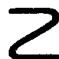
\includegraphics[keepaspectratio]{images/part001_8adf5445.jpg}}

and \(\operatorname{long}(\mathbf{M} / \mathfrak{q}\mathbf{M})\leqslant \operatorname{long}(\mathbf{M} / \mathfrak{x}\mathbf{M})\) ; the three cases

\[
e _ {\mathfrak {q}} (\mathrm{M}) <   \operatorname{long} (\mathrm{M} / \mathfrak {q} \mathrm{M}), e _ {\mathfrak {q}} (\mathrm{M}) = \operatorname{long} (\mathrm{M} / \mathfrak {q} \mathrm{M}), e _ {\mathfrak {q}} (\mathrm{M}) > \operatorname{long} (\mathrm{M} / \mathfrak {q} \mathrm{M})
\]

are possible (p.~106, exerc. 16 and 17).

\specialchapter{Exercises}
\setcounter{exercisesection}{0}

\exercisesection{KRULL DIMENSION OF A RING}

\begin{enumerate}
\def\labelenumi{\arabic{enumi})}
\tightlist
\item
  Let X be a topological space and Y a subspace of X. One says that Y is very dense in X if for every closed subset F of X, F is the closure of F ∩ Y.
\end{enumerate}

\begin{enumerate}
\def\labelenumi{\alph{enumi})}
\item
  For Y to be very dense in X, it is necessary and sufficient that for every nonempty locally closed subset F of X, F ∩ Y be nonempty.
\item
  If Y is very dense in X and Z is a subspace of Y very dense in X, then Z is very dense in X. If Y is very dense in X and F is a locally closed subset of X, then Y ∩ F is very dense in F.
\item
  If Y is very dense in X, one has \(\dim(\mathbf{Y}) = \dim(\mathbf{X})\) .
\end{enumerate}

\begin{enumerate}
\def\labelenumi{\arabic{enumi})}
\setcounter{enumi}{1}
\item
  Let A be a ring and Specmax(A) the set of maximal ideals of A. For Specmax(A) to be very dense in Spec(A), it is necessary and sufficient that A be a Jacobson ring (V, § 3, no. 4). One then has dim Specmax(A) = dim(A).
\item
  Show that if A is a Jacobson ring, A{[}{[}X{]}{]} is not a Jacobson ring. (Compare Specmax(A) and Specmax(A{[}{[}X{]}{]}).)
\item
  \begin{enumerate}
  \def\labelenumii{\alph{enumii})}
  \tightlist
  \item
    Show that one can associate in a unique way to every ordered set E an element of \(\{-\infty\}\cup\mathbf{N}\cup\{+\infty\}\) , denoted dev(E) (deviation of E), such that the following properties are satisfied:
  \end{enumerate}
\end{enumerate}

\(\alpha)\) We have \(\operatorname{dev}(\mathbf{E}) = -\infty\) if and only if the relation \(a \leqslant b\) in \(\mathbf{E}\) implies \(a = b\) .

β) Let n be a positive integer. The deviation of E is ≤ n if and only if, for every infinite decreasing sequence \((a_{k})_{k\in\mathbb{N}}\) of elements of E, one has \(\text{dev}([a_{k}, a_{k-1}]) \leqslant n - 1\) for all sufficiently large k.

\begin{enumerate}
\def\labelenumi{\alph{enumi})}
\setcounter{enumi}{1}
\item
  For one to have \(\text{dev}(\mathbf{E}) \leqslant 0\) , it is necessary and sufficient that every strictly decreasing sequence of elements of E be stationary. One has \(\text{dev}(\mathbf{N}) = 0\) , \(\text{dev}(\mathbf{Z}) = 1\) , \(\text{dev}(\mathbf{Q}) = +\infty\) .
\item
  If E and F are ordered sets and \(f: \mathbf{E} \to \mathbf{F}\) is a strictly increasing map, one has \(\operatorname{dev}(\mathbf{E}) \leqslant \operatorname{dev}(\mathbf{F})\) . We have \(\operatorname{dev}(\mathbf{E} \times \mathbf{F}) = \sup(\operatorname{dev}(\mathbf{E}), \operatorname{dev}(\mathbf{F}))\) .
\item
  Let S(E) be the set of infinite increasing stationary sequences of elements of E, ordered by the product order. Then one has \(\operatorname{dev}(\mathbf{S}(\mathbf{E})) = \operatorname{dev}(\mathbf{E}) + 1\) .
\end{enumerate}

\begin{enumerate}
\def\labelenumi{\arabic{enumi})}
\setcounter{enumi}{4}
\tightlist
\item
  If A is a ring (not necessarily commutative), M a left A-module, one denotes by Kdev(M) the deviation of the set of submodules of M, ordered by inclusion. One sets \(Kdev(A) = Kdev(A_s)\).
\end{enumerate}

\begin{enumerate}
\def\labelenumi{\alph{enumi})}
\tightlist
\item
  If N is a submodule of an A-module M, one has
\end{enumerate}

\[
\operatorname{Kdev} (\mathbf {M}) = \sup (\operatorname{Kdev} (\mathbf {N}), \operatorname{Kdev} (\mathbf {M} / \mathbf {N}))  .
\]

\begin{enumerate}
\def\labelenumi{\alph{enumi})}
\setcounter{enumi}{1}
\item
  Suppose A is commutative. If p and q are two prime ideals of A such that p ⊂ q and p ≠ q, one has dev(A/p) \textgreater{} dev(A/q). (Use the ideals p + Ax, where x is an element of q - p.) Deduce that dim(A) ≤ Kdev(A).
\item
  Suppose A is commutative and noetherian. Prove that one has dim(A) = Kdev(A) (reason by induction on dim(A), assuming that Kdev(B) ≤ dim(B) for every commutative noetherian ring B such that dim(B) \textless{} dim(A); let S be the set of s ∈ A that belong to none of the prime ideals p of A such that dim(A) = dim(A/p); show that, for every finitely generated A-module M such that \(S^{-1}M = 0\) , one has \(\mathrm{Kdev}(\bar{\mathrm{M}}) < \dim(\mathrm{A})\) using the fact that \(S^{-1}A\) is artinian, deduce that \(\mathrm{Kdev}(\mathrm{A}) \leqslant \dim(\mathrm{A})\) . Prove that we have \(\dim(\mathrm{M}) = \mathrm{Kdev}(\mathrm{M})\) for every finitely generated A-module M.
\end{enumerate}

6). a) Let A be a Noetherian (commutative) ring, m an ideal of A contained in the radical of A, and gr(A) the graded ring associated with the m-adic filtration of A. Associate to each ideal of A an ideal of gr(A), and deduce from this that Kdev(A) ≤ Kdev(gr(A)) (cf. Exercise 4, c)). Consequently, one has dim(A) ≤ dim(gr(A)) (Exercise 5, c)).

\begin{enumerate}
\def\labelenumi{\alph{enumi})}
\setcounter{enumi}{1}
\tightlist
\item
  Assume now that m = xA, where x belongs to the radical of A. Show that gr(A) is isomorphic to a quotient of the graded algebra (A/m)[T]. Show that the ordered set F of graded ideals of (A/m) {[}T{]} is isomorphic to the set of increasing sequences of ideals of A/m; deduce from this (exerc. 4, d)) that one has dev(F) = Kdev(A/(x)) + 1, then dim(A) ≤ dim(A/m) + 1.
\end{enumerate}

\begin{enumerate}
\def\labelenumi{\arabic{enumi})}
\setcounter{enumi}{6}
\tightlist
\item
  Let A be the ring of germs at 0 of functions of class \(C^\infty\) on \(\mathbf{R}_{+}\). We propose to show that the ring A is of infinite dimension. We denote by C the algebra of functions of class \(C^\infty\) on \(\mathbf{R}_{+}\) , and let F be the ideal formed by the functions vanishing in a neighborhood of 0, so that \(A = C / F\) .
\end{enumerate}

\begin{enumerate}
\def\labelenumi{\alph{enumi})}
\item
  Let \((x_{n})_{n\in \mathbb{N}}\) be a strictly decreasing sequence, tending to 0, of elements of \(\mathbf{R}_{+}\) , and let \(\mathfrak{U}\) be an ultrafilter on \(\mathbf{N}\) finer than the filter of complements of finite sets. Show that the set \(\mathbf{J}_1\) of \(f\in \mathbf{C}\) such that the set of \(n\in \mathbf{N}\) such that \(f(x_{n}) = 0\) belongs to \(\mathfrak{U}\) is a prime ideal of \(\mathbf{C}\) .
\item
  We denote by \(\tau_{n}(f)\) the function \(x\mapsto f(x + x_{n})\) . Show that if J is a prime ideal of C, the set \(\varphi(J)\) of \(f\) such that the set of \(n\in\mathbf{N}\) with \(\tau_{n}f\in\mathbf{J}\) belongs to \(\mathfrak{U}\) is a prime ideal of C.
\item
  One defines a sequence \(\mathbf{I}_n\) of ideals of C by \(\mathbf{I}_0 = \mathbf{J}_1\) , \(\mathbf{I}_{n+1} = \varphi(\mathbf{I}_n)\) . Show that \((\mathbf{I}_n)_{n\in\mathbb{N}}\) is a strictly decreasing sequence of prime ideals of C containing F.
\end{enumerate}

\begin{enumerate}
\def\labelenumi{\arabic{enumi})}
\setcounter{enumi}{7}
\item
  Let X be a topological space. Show that the map \(x \mapsto \dim_x(X)\) from X to \(\overline{\mathbf{R}}\) is upper semicontinuous.
\item
  Let A be a ring, p a prime ideal of A, and M a finitely generated A-module. Show that one has:
\end{enumerate}

\[
\dim_ {\mathbf {A} _ {\mathfrak {p}}} (\mathbf {M} _ {\mathfrak {p}}) + \dim_ {\mathbf {A} / \mathfrak {p}} (\mathbf {M} / \mathfrak {p} \mathbf {M}) \leqslant \dim_ {\mathbf {A}} (\mathbf {M}).
\]

\begin{enumerate}
\def\labelenumi{\arabic{enumi})}
\setcounter{enumi}{9}
\tightlist
\item
  A ring A is said to be equidimensional if all irreducible components of Spec(A) have the same dimension. Let A be a ring and n an integer. The following conditions are equivalent:
\end{enumerate}

\begin{enumerate}
\def\labelenumi{\alph{enumi})}
\tightlist
\item
  every chain of prime ideals of A is contained in a chain of length n;
\item
  for every maximal ideal m of A, the ring A \(_{m}\) is equidimensional, catenary, and of dimension n.
\end{enumerate}

\begin{enumerate}
\def\labelenumi{\arabic{enumi})}
\setcounter{enumi}{10}
\tightlist
\item
  Let \((\mathbf{A}_{i}, f_{ij})\) be an inductive system of rings relative to a filtered ordered set I, with inductive limit A. Show that one has \(\dim(\mathbf{A}) \leqslant \lim.\inf\dim(\mathbf{A}_{i})\) and that one has equality when the homomorphisms \(f_{ij}\) are faithfully flat. Give an example where the homomorphisms \(f_{ij}\) are flat and where one has \(\dim(\mathbf{A}) < \lim.\inf\dim(\mathbf{A}_{i})\) (take I = N, \(A_{n} = Z[n^{-1}]\) , A = Q).
\end{enumerate}

Let A be a ring, and let I and J be two ideals of A. Suppose that for every maximal ideal m of A, we have IA \(_{m}\) = JA \(_{m}\) . Deduce from this that I = J.

\begin{enumerate}
\def\labelenumi{\alph{enumi})}
\setcounter{enumi}{1}
\item
  Let A be a ring such that, for every maximal ideal m of A, the ring \(\mathrm{A}_{\mathfrak{m}}\) is Noetherian and such that, for every nonzero element \(f\) of A, there exist only finitely many maximal ideals of A containing \(f\) . Then A is Noetherian. (Let \(a\) be an ideal of A. We will first show that there exists a finite family \((x_1, ..., x_n)\) of elements of \(a\) such that the maximal ideals of A that contain \(\{x_1, ..., x_n\}\) contain \(a\). We will then construct a finite family of elements \(y_1, ..., y_l\) such that for every maximal ideal m of A, \(\{y_1, ..., y_l\}\) generates the ideal \(a\mathrm{A}_{\mathfrak{m}}\) of \(\mathrm{A}_{\mathfrak{m}}\) . We conclude by using a).
\item
  Let A be a semi-local ring such that, for every maximal ideal m, the ring \(A_{m}\) is Noetherian. Then A is Noetherian.
\end{enumerate}

\begin{enumerate}
\def\labelenumi{\arabic{enumi})}
\setcounter{enumi}{12}
\item
  Let K be a field, \((n_{r})_{r\geqslant1}\) a strictly increasing sequence of integers \textgreater0; for every integer \(i\geqslant0\) , denote by \(p_{i}\) the ideal of the ring \(\mathrm{K}[(\mathrm{X}_{j})_{j\in\mathbb{N}}]\) generated by the \(X_{j}\) for \(n_{1}+\cdots+n_{i}\leqslant j<n_{1}+\cdots+n_{i}+n_{i+1}\) , and let S be the set of elements of \(\mathrm{K}[(\mathrm{X}_{j})]\) that belong to none of the \(p_{i}\). Then the ring \(S^{-1}K[(X_{j})]\) is Noetherian and of infinite dimension (use Exercise 12 to show that \(S^{-1}K[(X_{j})]\) is Noetherian) \(^{1}\) .
\item
  Let V be a discrete valuation ring, and let \(\pi\) be a uniformizer of V. In the ring V{[}T{]}, the ideal \(m_1 = (\pi T - 1)\) is maximal and of height 1, the ideal \(m_2 = (\pi) + (T)\) is maximal and of height 2. The fields V{[}T{]}/ \(m_1\) and V{[}T{]}/ \(m_2\) are isomorphic to the field of fractions of V and to the residue field of V, respectively. One has \(\dim(\mathrm{V}[T]) = 2\), but \(\dim(\mathrm{V}[T]/m_1) + \dim(\mathrm{V}[T]_{m_1}) = 1\) and \(\dim(\mathrm{gr}_{m_1}(\mathrm{V}[T])) = 1\).
\end{enumerate}

With the notation of the preceding exercise, suppose that the residue field and the field of fractions of the ring V are isomorphic (this is the case, for example, when \(\mathrm{V} = k[[\mathrm{U}]]\) , the field \(k\) being the field of fractions of a ring of formal power series in infinitely many indeterminates with coefficients in a field). Let \(\sigma\) be an isomorphism of \(\mathrm{V[T] / m_1}\) onto \(\mathrm{V[T] / m_2}\) . Let C denote the subring of \(\mathrm{V[T]} = \mathrm{E}\) consisting of the elements of E whose classes modulo \(m_1\) and \(m_2\) correspond under \(\sigma\) . Show that C is Noetherian and that \(m_1m_2 = m_1 \cap m_2\) is a maximal ideal of C. Show that E is the integral closure of C (noting that \(\mathrm{E} = \mathrm{C} + \mathrm{C}\cdot(\pi T - 1)\) and that \((\pi T - 1)^2 + (\pi T - 1)\) belongs to C).

Let \(\mathring{\mathrm{A}}\) be the local ring \(\mathbf{C}_{\mathfrak{m}_1\mathfrak{m}_2}\) . Then A is an integral domain of dimension 2, hence catenary; the integral closure \(\mathbf{B} = \mathbf{E} \otimes_{\mathbb{C}} \mathbf{A}\) of \(\mathring{\mathrm{A}}\) is a semi-local Noetherian ring having exactly two maximal ideals \(\mathfrak{n}_1\) and \(\mathfrak{n}_2\) , and we have \(\dim(\mathbf{B}_{\mathfrak{n}_1}) = 1\) , \(\dim(\mathbf{B}_{\mathfrak{n}_2}) = 2\) .

¶ 16) We keep the notation of the preceding exercise, and we identify B with the quotient of the polynomial ring A{[}U{]} by the prime ideal \(\mathfrak{p}\) generated by \(U^2 + U - \pi T(\pi T - 1)\). Let \(\mathfrak{q}_i\) be the ideal of A{[}U{]} such that \(\mathfrak{n}_i = \mathfrak{q}_i/\mathfrak{p}\). Then \(\operatorname{ht}(\mathfrak{q}_i) = 3\), \(\operatorname{ht}(\mathfrak{p}) = 1\), and the chain \(\mathfrak{p} \subset \mathfrak{q}_1\) is saturated. In particular, A{[}U{]} and A{[}U{]}\(_{\mathfrak{q}_1}\) are not catenary.

\begin{enumerate}
\def\labelenumi{\arabic{enumi})}
\setcounter{enumi}{16}
\tightlist
\item
  \begin{enumerate}
  \def\labelenumii{\alph{enumii})}
  \tightlist
  \item
    Let A be an integral domain and \(f \in \mathrm{A}[\mathrm{T}], f \neq 0\). Show that there exists a maximal ideal m of \(\mathrm{A}[\mathrm{T}]\) such that \(f \notin \mathfrak{m}\) (take a maximal ideal containing T.f-1).
  \end{enumerate}
\end{enumerate}

\begin{enumerate}
\def\labelenumi{\alph{enumi})}
\setcounter{enumi}{1}
\tightlist
\item
  Let A be a ring. Show that one has dim(Specmax(A{[}T{]})) \(\geqslant\) dim(A) + 1. (Let \(\mathfrak{p}_0\subset \mathfrak{p}_1\subset \cdots \subset \mathfrak{p}_n\) be a chain of prime ideals of A. Consider the chain
\end{enumerate}

\[
\mathfrak {p} _ {0} [ \mathrm{T} ] \subset \mathfrak {p} _ {1} [ \mathrm{T} ] \subset \mathfrak {p} _ {2} [ \mathrm{T} ] \dots \subset \mathfrak {p} _ {n} [ \mathrm{T} ] \subset (\mathfrak {p} _ {n}, \mathrm{T})
\]

of prime ideals of A{[}T{]} and let us set

\[
\left\{ \begin{array}{l} \mathrm{U} _ {i} = \mathrm{V} (\mathfrak {p} _ {i} [ \mathrm{T} ]) \cap \operatorname{Specmax} (\mathrm{A} [ \mathrm{T} ]), \quad 0 \leqslant i \leqslant n \\ \mathrm{U} _ {n + 1} = \mathrm{V} (\mathfrak {p} _ {n}, \mathrm{T}) \cap \operatorname{Specmax} (\mathrm{A} [ \mathrm{T} ]). \end{array} \right.
\]

Show, using \(a\) ) that \((\mathrm{U}_i)_{0 \leqslant i \leqslant n+1}\) is a strictly increasing sequence of irreducible closed subsets of Specmax (A{[}T{]}).

\begin{enumerate}
\def\labelenumi{\alph{enumi})}
\setcounter{enumi}{2}
\tightlist
\item
  Let \(k\) be a field, and let S be the subset of \(k[\mathrm{X}, \mathrm{Y}]\) formed by the elements of the form \(1 + \mathrm{X}g(\mathrm{X}, \mathrm{Y})\) , and let \(\mathrm{A} = \mathrm{S}^{-1}k[\mathrm{X}, \mathrm{Y}]\) .
\end{enumerate}

Show that one has dim(Specmax(A)) = 1 and dim(Spec(A)) = 2. Generalize to the case of several indeterminates.

\begin{enumerate}
\def\labelenumi{\alph{enumi})}
\setcounter{enumi}{3}
\item
  Show that for every pair of integers \(0 \leqslant n < m\) , there exists a Noetherian ring A such that \(\dim(\text{Specmax}(A)) = n\) and \(\dim(\text{Specmax}(A[T])) = m\) .
\item
  Let A be the Noetherian ring defined in exerc. 13. Show that one has dim(Specmax(A)) = 1 and dim(Specmax(A{[}T{]})) = \(\infty\) .
\end{enumerate}

\exercisesection{DIMENSION OF ALGEBRAS}

\begin{enumerate}
\def\labelenumi{\arabic{enumi})}
\item
  Let V be a discrete valuation ring, with fraction field K, and let n be an integer. Let A be the subring of the polynomial ring \(K[X_{1},...,X_{n}]\) formed by the polynomials whose constant term lies in V. The canonical homomorphism from V to A satisfies property (PM) and the canonical homomorphism \(V/m_{V} \rightarrow A/m_{V}A\) is an isomorphism. Moreover, one has \(\dim(A) \geqslant n + 1\) and \(\dim(V) = 1\) . As soon as \(n \geqslant 1\) , one therefore has \(\dim(A) > \dim(V) + \dim(A/m_{V}A)\) . Show that A is not Noetherian. Using formal series, construct an analogous example where A is local and not Noetherian.
\item
  Let V be a discrete valuation ring, with fraction field K and residue field k. Denote by A the ring \(K \times k\) and \(\rho : V \to A\) the homomorphism deduced from the canonical homomorphisms from V to K and k. The homomorphism \(\rho\) is injective, the map \(^{a}\rho : \text{Spec}(A) \to \text{Spec}(V)\) is surjective, A is a finitely generated V-algebra, and we have \(\dim(A) < \dim(V)\) .
\item
  Let A be an integral domain of dimension 1, and let \(\mathfrak{p}_0 \subset \mathfrak{p}_1 \subset \mathfrak{p}_2\) be three distinct nonzero prime ideals of A{[}X{]}. Show that we have \(\mathfrak{p}_0 \cap \mathbf{A} = \{0\}\) , \(\mathfrak{p}_1 = (\mathfrak{p}_1 \cap \mathbf{A})\cdot\mathrm{A}{[}X{]}\), and that \(\mathfrak{p}_2\) is a maximal ideal of A{[}X{]}.
\item
  Let A be a local integrally closed ring, \(m_A\) its maximal ideal and K its field of fractions. For every element x of K, we denote by A{[}x{]} the sub-A-algebra of K generated by x. Let x be an element of K* such that \(x^{-1}\) does not belong to A. Let A{[}X{]} be the ring of polynomials in one indeterminate X, with coefficients in A, and \(\varphi\) the evaluation map P \(\mapsto\) P(x) of A{[}X{]} on A{[}x{]}.
\end{enumerate}

\begin{enumerate}
\def\labelenumi{\alph{enumi})}
\item
  The kernel of \(\varphi\) is the ideal Q generated by the polynomials of the form \(aX + b\) , where \(a, b \in A\) and \(ax + b = 0\) . (If \(\mathrm{P}(X) = \sum_{i=0}^{n} a_i X^i\) is such that \(\mathrm{P}(x) = 0\) , note that then \(-b_0 = a_0 x\) is integral over \(A\) therefore belongs to \(A\) .)
\item
  The ideal \(m_A A[x]\) of \(A[x]\) is prime, and it is maximal if and only if \(x\) belongs to \(A\) .
\end{enumerate}

\begin{enumerate}
\def\labelenumi{\arabic{enumi})}
\setcounter{enumi}{4}
\item
  Let A be an integrally closed ring with fraction field K. Given a prime ideal p of A, and an element x of K such that \(x \notin A_{p}\) , and \(x^{-1} \notin A_{p}\) the ideal pA{[}x{]} of A{[}x{]} is prime; we have: pA{[}x{]} ∩ A = p and the canonical homomorphism (A/p){[}X{]} → A{[}x{]}/pA{[}x{]} is an isomorphism.
\item
  \begin{enumerate}
  \def\labelenumii{\alph{enumii})}
  \tightlist
  \item
    Using the previous exercises, show that if A is an integral domain of dimension 1, then dim(A{[}X{]}) = 2 if and only if all the localizations at a prime ideal of the integral closure of A are valuation rings.
  \end{enumerate}
\end{enumerate}

\begin{enumerate}
\def\labelenumi{\alph{enumi})}
\setcounter{enumi}{1}
\tightlist
\item
  Show that if one has \(\dim(\mathbf{A}) = n\) and \(\dim(\mathbf{A}[\mathbf{X}]) > n + 1\), there exists a prime ideal \(\mathfrak{p}\) of A such that \(\operatorname{ht}(\mathfrak{p}) = 1\) and either \(\dim(\mathbf{A}_{\mathfrak{p}}[\mathbf{X}]) > 2\) or \(\dim((\mathbf{A}/\mathfrak{p})[\mathbf{X}]) > \dim(\mathbf{A}/\mathfrak{p}) + 1\) .
\item
  Deduce that if A is Prüferian (VII, § 2, exerc. 12), then we have \(\dim(\mathbf{A}[\mathbf{X}_1, ..., \mathbf{X}_n]) = \dim(\mathbf{A}) + n\) , for every integer \(n \geqslant 0\) .
\end{enumerate}

\begin{enumerate}
\def\labelenumi{\arabic{enumi})}
\setcounter{enumi}{6}
\item
  Let B be an integrally closed ring, with field of fractions L. We set \(d = \dim(B)\) and \(t = \dim(B[X])\) . Let L' be a non-trivial extension of L in which L is algebraically closed, and let V be a discrete valuation ring (which is not a field) having L' as its residue field. We denote by K the field of fractions of V and by A the set of elements of V whose image in L' under the canonical homomorphism V → L' belongs to B. The ring A is integrally closed with field of fractions K. Let p denote the kernel of the surjective homomorphism A → B. Show that every non-zero prime ideal of A contains p, whence dim(A) = dim(B) + 1. Considering an element x of V whose image in L' does not belong to L, show that the ring of fractions A \(_{p}\) is not a valuation ring, and that pA \(_{p}\) {[}x{]} is not minimal among the non-zero prime ideals of A \(_{p}\) {[}x{]}. Using exercise 6, deduce that one has dim(A{[}x{]}) ≥ t + 2. Conclude that one has dim(A{[}x{]}) = t + 2 by a direct argument. Finally show that for every pair (d, t) of integers with d + 1 ≤ t ≤ 2d + 1, there exists an integral domain A of dimension d such that dim(A{[}X{]}) = t.
\item
  Show that the polynomial ring A{[}X{]} is a faithfully flat A-module, that for every maximal ideal m of A one has dim(A{[}X{]}/mA{[}X{]}) = 1, and deduce from the preceding exercise the existence of ring homomorphisms \(\rho: A \to B\) satisfying condition (PM) and such that \(\dim(B) > \dim(A) + \inf_{\mathfrak{m}\in S}\dim(B/\mathfrak{m}B)\) (where S is the set of maximal ideals of A).
\item
  Let A be an integral domain and B an integral domain containing A and integral over A. Let p be a prime ideal of A such that the integral closure of the ring of fractions \(A_{p}\) is a local ring. For every prime ideal q of B lying over p, one has ht(q) = ht(p) (use V, § 2, n° 1, prop. 2).
\end{enumerate}

¶ 10) a) Let A be an integral domain, K its field of fractions, and m a positive integer. Let \(t_1, \ldots, t_m\) be elements of K and \(\varphi: \mathrm{A}[\mathrm{X}_1, \ldots, \mathrm{X}_m] \to \mathrm{A}[t_1, \ldots, t_m]\) the unique homomorphism of A-algebras such that \(\varphi(\mathrm{X}_i) = t_i\) . Show that the height of the kernel ideal of \(\varphi\) is equal to m. b) Deduce that for every \(m\) -tuple ( \(t_1, \ldots, t_m\) ) of elements of K, one has \(\dim(\mathrm{A}[t_1, \ldots, t_m]) \leqslant \dim(\mathrm{A}[\mathrm{X}_1, \ldots, \mathrm{X}_m]) - m\) .

¶ 11) Let A be an integral domain and K its field of fractions. Let \((0) \subset \mathfrak{p}_1 \subset \ldots \subset \mathfrak{p}_h\) be a chain of prime ideals of A. Show that there exists a valuation ring V of K and a chain of prime ideals \((0) \subset \mathfrak{q}_1 \subset \ldots \subset \mathfrak{q}_h\) of V such that \(\mathfrak{q}_i \cap A = \mathfrak{p}_i\) . (Proceed by induction on \(h\) , reducing to the case where A is a local ring and using, for the case \(h = 1\) , exercise 7 of VI, § 1.)

\begin{enumerate}
\def\labelenumi{\arabic{enumi})}
\setcounter{enumi}{11}
\tightlist
\item
  \begin{enumerate}
  \def\labelenumii{\alph{enumii})}
  \tightlist
  \item
    Let A and K be as above, let B be an integral domain containing A and integral over A, and let L be the fraction field of B. Let \(k \geqslant 0\) be an integer. If, for every \(m\)-tuple \((t_1, \ldots, t_m)\) of elements of L, we have \(\dim(A[t_1, \ldots, t_m]) \leqslant k\), then, for every \(m\)-tuple \((u_1, \ldots, u_m)\) of elements of L, we have \(\dim(B[u_1, \ldots, u_m]) \geqslant k\). b) Let p be a prime ideal of A. Show that if, for all \(m\)-tuples \((t_1, \ldots, t_m)\) of elements of K, one has \(\dim(A[t_1, \ldots, t_m]) \leqslant k\), then we have for all \(m\)-tuples \((s_1, \ldots, s_m)\) of elements of the field of fractions of A/p, the inequality \(\dim((A/p)[s_1, \ldots, s_m]) \leqslant k - \text{ht}(p)\) .
  \end{enumerate}
\end{enumerate}

¶ 13) Let A be an integral domain and K its field of fractions. For every integer \(k \geqslant 0\) , the following properties are equivalent:

\begin{enumerate}
\def\labelenumi{(\roman{enumi})}
\item
  Every subring B of K containing A has dimension \(\leqslant k\) .
\item
  Every valuation ring V of K containing A has dimension \(\leqslant k\) .
\item
  For every choice of \(k\) elements \(t_1, \ldots, t_k\) of \(\mathbf{K}\) , one has \(\dim(A[t_1, \ldots, t_k]) \leqslant k\) .
\item
  We have \(\dim(A[X_1, ..., X_m]) \leqslant k + m\) for every integer \(m \geqslant 0\) .
\end{enumerate}

\begin{enumerate}
\def\labelenumi{\arabic{enumi})}
\setcounter{enumi}{13}
\tightlist
\item
  Let A be an integral domain, with field of fractions K, and \(m \in N\). Show that we have
\end{enumerate}

\[
\dim (\mathrm{A} [ \mathrm{X} _ {1},..., \mathrm{X} _ {m} ]) = m + \sup \left\{\dim (\mathrm{A} [ t _ {1},..., t _ {m} ]) | t _ {i} \in \mathrm{K}, 1 \leqslant i \leqslant m \right\}.
\]

(We will use Exercise 10). More generally, if F is a field, an extension of K, show that we have

\[
\dim \left(\mathrm{A} \left[ \mathrm{X} _ {1}, \dots , \mathrm{X} _ {m} \right]\right) = \sup \left\{\dim (\mathrm{A} \left[ t _ {1}, \dots , t _ {m} \right]) \mid t _ {i} \in \mathrm{F}, 1 \leqslant i \leqslant m \right\} + \sup (0, m - \deg . \operatorname{tr} _ {\mathbf {K}} (\mathrm{F})).
\]

\begin{enumerate}
\def\labelenumi{\arabic{enumi})}
\setcounter{enumi}{14}
\tightlist
\item
  With the notations of the previous exercises, show that if for some integer \(k \geqslant 0\) , one has \(\dim(A[X_1, ..., X_m]) \geqslant k + m + 1\) for a suitable integer \(m\), one has the inequality \(\dim(A[X_1, ..., X_k]) \geqslant 2k + 1\) .
\end{enumerate}

  ¶ 16) Let A be an integral domain and K its field of fractions. One calls the valuative dimension of A and denotes it by \(\dim_{\mathrm v}(\mathrm A)\) the real number \(\sup_{A \subset V \subset K} \dim(V)\) , where V ranges over the set of valuation rings of K containing A

\begin{enumerate}
\def\labelenumi{\alph{enumi})}
\item
  Show that one has \(\dim(\mathrm A) \leqslant \dim_{\mathrm v}(\mathrm A)\) (exercise 11).
\item
  If A is Prüferian (VII, § 2, exerc. 12), show that one has \(\dim(\mathrm A) = \dim_{\mathrm v}(\mathrm A)\).
\item
  Show that, for all \(m \in \mathbf{N}\) , one has
\end{enumerate}

\[
\dim_ {\mathbf {v}} (\mathrm{A} [ \mathrm{X} _ {1},..., \mathrm{X} _ {m} ]) = \dim_ {\mathbf {v}} (\mathrm{A}) + m.
\]

(Note that a valuation ring is Prüferian, and one will use b) and exercise 6, p.~84.)

\begin{enumerate}
\def\labelenumi{\alph{enumi})}
\setcounter{enumi}{3}
\tightlist
\item
  Show that if one has \(\dim_{\mathrm v}(\mathrm A) = s < \infty\), one has, for every integer \(m \geqslant s - 1\) the equality
\end{enumerate}

\[
\dim (\mathrm{A} [ \mathrm{X} _ {1},..., \mathrm{X} _ {m} ]) = m + s.
\]

\begin{enumerate}
\def\labelenumi{\alph{enumi})}
\setcounter{enumi}{4}
\tightlist
\item
  Let \(s \in \mathbf{N}\) . Show that we have \(\dim_{\mathrm{v}}(\mathbf{A}) = s\) if and only if \(\dim(\mathbf{A}[\mathbf{X}_1, ..., \mathbf{X}_s]) = 2s\) (using \(d\) ) and Exercises 13 and 14).
\end{enumerate}

Deduce that, for every integral Noetherian ring A, one has \(\dim(\mathrm{A}) = \dim_{\mathrm{v}}(\mathrm{A})\).

\begin{enumerate}
\def\labelenumi{\arabic{enumi})}
\setcounter{enumi}{16}
\tightlist
\item
  Let A be an integral domain. Set \(n_k(A) = \dim(A[X_1, ..., X_k])\) for every integer \(k \geqslant 0\). Let D be the set of sequences of integers \((n_i)_{i \geqslant 0}\) such that there exists an integral domain A with \(n_i = n_i(A)\) for every integer \(i \geqslant 0\) .
\end{enumerate}

\begin{enumerate}
\def\labelenumi{\alph{enumi})}
\tightlist
\item
  Prove the inequalities
\end{enumerate}

\[
\sup \left(n _ {0} (\mathrm{A}) + i + 1, n _ {i} (\mathrm{A}) + 1\right) \leqslant n _ {i + 1} (\mathrm{A}) \leqslant \inf \left(2 n _ {i} (\mathrm{A}) + 1, 2 ^ {i + 1} \left(n _ {0} (\mathrm{A}) + 1\right) - 1\right).
\]

\begin{enumerate}
\def\labelenumi{\alph{enumi})}
\setcounter{enumi}{1}
\tightlist
\item
  Show that the only sequence of integers beginning with 1, 2 and belonging to D is the sequence \(n_{i}=i+1\) . (Let A be such that \(n_{0}(A)=1\) , \(n_{1}(A)=2\) . By exerc. 6, p.~84, the integral closure of A is Prüferian. Use exerc. 6, c), p.~84 to conclude.)\\
\item
  Prove the inequalities
\end{enumerate}

\[
n _ {0} (\mathrm{A}) + i \leqslant n _ {i} (\mathrm{A}) \leqslant (n _ {0} (\mathrm{A}) + 1) (i + 1) - 1.
\]

Deduce that if one has \(n_0(\mathbf{A}) = 0\) , then we have \(n_i(\mathbf{A}) = i\) for every \(i \in \mathbf{N}\) .

\begin{enumerate}
\def\labelenumi{\alph{enumi})}
\setcounter{enumi}{3}
\item
  Show that the sequence of differences \(n_{i+1}(\mathbf{A}) - n_i(\mathbf{A})\) is stationary.
\item
  We use the notations of exerc. 7, p.~84. Let δ be the transcendence degree of L' over L. Then:
\end{enumerate}

\begin{enumerate}
\def\labelenumi{(\roman{enumi})}
\item
  If \(\delta = 0\) , one has \(n_i(A) = n_i(B) + 1\) for every \(i\) .
\item
  If \(1 \leqslant \delta < \infty\) , one has \(n_i(A) = n_i(B) + i + 1\) for \(0 \leqslant i \leqslant \delta\) and \(n_i(A) = n_i(B) + \delta + 1\) for \(i \geqslant \delta\) .
\item
  If \(\delta = \infty\) , one has \(n_i(A) = n_i(B) + i + 1\) for every \(i\) .
\end{enumerate}

(For a characterization of the elements of D, one may consult T. Parker, Amer. J. Math., 97 (1975), pp. 308–311.)

* 18) Let A (resp. B) denote the algebra C \(\{z_{1}, z_{2}, z_{3}\}\) (resp. C \(\{u, v\}\) ) of convergent series in the variables \(z_{1}, z_{2}, z_{3}\) (resp. \(u, v\) ) and \(\varphi: A \to B\) the unique algebra homomorphism such that \(\varphi(z_{1}) = uv\) , \(\varphi(z_{2}) = v(e^{u} - 1)\) , \(\varphi(z_{3}) = v\) . Show that \(\varphi\) is injective, and that we have dim(A) = 3 and dim(B) = 2. *

\exercisesection{DIMENSION OF NOETHERIAN RINGS}

\begin{enumerate}
\def\labelenumi{\arabic{enumi})}
\tightlist
\item
  Let A be a ring, and let U be an open subset of Spec(A).
\end{enumerate}

\begin{enumerate}
\def\labelenumi{\alph{enumi})}
\item
  Show that the map \(\mathfrak{p} \mapsto \mathrm{V}(\mathfrak{p}) \cap \mathrm{U}\) induces a bijection from U onto the set of closed irreducible subsets of U.
\item
  Show that dim(U) is the upper bound of the set of lengths of chains of prime ideals of A belonging to U.
\item
  Let \(\Phi\) be the set of minimal prime ideals of A belonging to U. Show that one has
\end{enumerate}

\[
\dim (\mathrm{U}) = \sup _ {\mathfrak {p} \in \Phi} \dim (\mathrm{V} (\mathfrak {p}) \cap \mathrm{U}).
\]

\begin{enumerate}
\def\labelenumi{\alph{enumi})}
\setcounter{enumi}{3}
\item
  Assume henceforth that A is local and U ≠ Spec(A). If A is Noetherian, establish the equality \(\dim(\mathrm{U}) = \sup_{\mathfrak{p}\in\Phi}(\dim(\mathrm{A}/\mathfrak{p}) - 1)\).
\item
  Let h be an integer such that 0 \textless{} h \textless{} dim(A). Let \(E_{h}\) be the set of prime ideals \(p \in U\) such that \(ht(p) = h\) and \(\dim(A/p) = \dim(A) - h\) . If A is Noetherian, show that \(E_{h}\) is infinite. Show that \(E_{h}\) may be finite when A is not Noetherian (take for A a valuation ring of height 2, for U the open \(\text{Spec}(A) - \{m_{A}\}\) , and choose h = 1).
\end{enumerate}

\begin{enumerate}
\def\labelenumi{\arabic{enumi})}
\setcounter{enumi}{1}
\item
  Let A be a Noetherian integral domain. Suppose that A is not a field and that the field of fractions of A is a finitely generated A-algebra. Then A is semi-local and of dimension 1. (Show that there exists a nonzero, non-invertible element \(f\) of A such that \(A[f^{-1}]\) is a field, and reduce to proving that \(\dim(A/(f)) = 0\) ; if it were otherwise, \(A/(f)\) would possess a prime ideal of height 1 whose inverse image p in A would be a prime ideal of height 2; but the local ring \(A_p\) of dimension 2 could have only a finite number of prime ideals, contrary to prop. 6 of § 3, no. 3.)
\item
  \begin{enumerate}
  \def\labelenumii{\alph{enumii})}
  \tightlist
  \item
    Let A be a Noetherian local ring, and let p be a prime ideal of A. Prove the inequality \(\dim_{\mathfrak{p}}(\mathbf{A}) \geqslant \mathrm{ht}(\mathfrak{p}) + \dim(\mathbf{A}/\mathfrak{p}) - 1\) .
  \end{enumerate}
\end{enumerate}

\begin{enumerate}
\def\labelenumi{\alph{enumi})}
\setcounter{enumi}{1}
\tightlist
\item
  Prove that there exists a Noetherian local ring R of dimension 3 having a prime ideal q such that ht(q) = 1 and dim(R/q) = 1. (Use exerc. 16, p.~83, by taking \(\mathbf{R} = \mathbf{A}[\mathbf{U}]_{\mathbf{q}}\) , and q = pR.) Let \(f \in \mathfrak{m}_{\mathbb{R}} - \mathfrak{q}\) ; show that \(\dim(\mathbf{R}_{f}) = 2\) (use exerc. 1, p.~86); we therefore have \(\dim_{\mathfrak{q}}(\mathbf{R}) = 2\) whereas \(\operatorname{ht}(\mathfrak{q}) + \dim(\mathbf{R}/\mathfrak{q}) - 1 = 1.\)
\end{enumerate}

\begin{enumerate}
\def\labelenumi{\arabic{enumi})}
\setcounter{enumi}{3}
\item
  Let \(k\) be a field, and let \(n\) be an integer \(\geqslant 1\). For each integer \(r \in [0, n]\) , let \(M_r\) be the vector subspace of \(k(X_1, ..., X_n)\) generated by the monomials \(X_1^{\alpha_1}\ldots X_r^{\alpha_r}\) with \(\alpha_1, ..., \alpha_r\) in \(Z\) and \(\alpha_r > 0\) . Put \(a_r = M_r + \cdots + M_n\) , for \(0 \leqslant r \leqslant n + 1\) . Then \(a_0\) is a subring of \(k(X_1, ..., X_n)\) , and the \(a_r\) are prime ideals of \(a_0\) . Put \(A = (a_0)_{a_1}\) and \(p_r = (a_r)_{a_1}\) for \(1 \leqslant r \leqslant n + 1\) . Show that the only prime ideals of the local ring \(A\) are the \(p_r\) , and that one has \(ht(p_r) = n + 1 - r\) and \(dim(A) = n\) . Moreover \(p_1\) is principal.
\item
  Let \(\rho: \mathbf{A} \to \mathbf{B}\) be a local homomorphism of complete Noetherian local rings, such that \([\kappa(\mathbf{B}): \kappa(\mathbf{A})] < \infty\) . Put \(n = \dim(\mathbf{B}/\mathfrak{m}_{\mathbf{A}}\mathbf{B})\) ; show that there exists a local A-homomorphism \(u: \mathbf{A}[[\mathbf{T}_1, ..., \mathbf{T}_n]] \to \mathbf{B}\) which makes B a \(\mathbf{A}[[\mathbf{T}_1, ..., \mathbf{T}_n]]\) -finite algebra. (Lift in B a maximal secant sequence of \(\mathbf{B}/\mathfrak{m}_{\mathbf{A}}\mathbf{B}\) and use III, § 3, exerc. 18.)
\item
  Let \(k\) be a field and A the ring of formal power series \(k[[X_1, X_2]]\) . Consider an ideal \(\mathfrak{n}\) of A containing a power of the maximal ideal \(\mathfrak{m}\) of A, and the ideal I generated by \((X_1 - X_2)\mathfrak{n}\) . Let M be the module A/I. Show that the sequence \((X_1)\) is secant for M without being completely secant for M.
\item
  Let A be a local, integral, Noetherian, non-catenary ring of dimension 3 (exerc. 16, p.~83), p ⊂ A a prime ideal such that ht(p) = 1, dim(A/p) = 1. Show that there exists an element x ∈ p such that p is minimal among the prime ideals containing Ax. Deduce that V(x) has an irreducible component of dimension 1.
\end{enumerate}

\exercisesection{HILBERT-SAMUEL SERIES}

\begin{enumerate}
\def\labelenumi{\arabic{enumi})}
\tightlist
\item
  Let \(\Gamma\) be a commutative group and let H be a graded ring of type \(\Gamma\) (A, II, p.~164).
\end{enumerate}

For \(\gamma\in\Gamma\) , we denote by H \(_{\gamma}\) the homogeneous component of degree \(\gamma\) of H. We assume that H is generated by H \(_{0}\) and a finite family (x \(_{i}\) ) \(_{i\in I}\) of homogeneous elements of degree \(\neq0\) . We denote by \(\gamma_{i}\) the degree of x \(_{i}\) . For every commutative group K, we denote by K{[}{[}Γ{]}{]} the product group K \(^{\Gamma}\) and we denote by \(\sum_{\gamma\in\Gamma}m_{\gamma}\text{T}^{\gamma}\) the element (m \(_{\gamma}\) ) of K \(^{\Gamma}\) . We denote by K{[}Γ{]} the subgroup K \(^{(\Gamma)}\) of K{[}{[}Γ{]}. We endow K{[}{[}Γ{]}{]} with its natural structure as a module over the algebra Z{[}Γ{]} of the group Γ. Finally, let C be a hereditary set of classes of H₀-modules (A, VIII, § 10, no. 1, def. 1) and let K(C) be the corresponding Grothendieck group (loc. cit., no. 2). For every H₀-module E of type C, we denote {[}E{]} its class in K(C).

\begin{enumerate}
\def\labelenumi{\alph{enumi})}
\tightlist
\item
  Suppose \(\mathbf{H}_0\) is Noetherian, and let \(\mathbf{M}\) be a finitely generated graded H-module such that for every \(\gamma \in \Gamma\) , the \(\mathbf{H}_0\) -module \(\mathbf{M}_{\gamma}\) is of type C. Show that the element \(\prod_{i \in I} (1 - T^{\gamma_i}) \sum_{\gamma \in \Gamma} [\mathbf{M}_{\gamma}] T^{\gamma}\) of
\end{enumerate}

\(K(\mathbb{C})[[\Gamma]]\) belongs to \(K(\mathbb{C})[\Gamma]\) .

\begin{enumerate}
\def\labelenumi{\alph{enumi})}
\setcounter{enumi}{1}
\tightlist
\item
  Suppose now that \(\Gamma = \mathbf{Z}^s\) , \(\mathrm{H}_{\gamma} = 0\) and \(\mathbf{M}_{\gamma} = 0\) for \(\gamma \notin \mathbf{N}^s\) , and that the \(\gamma_i\) are basis vectors of \(\mathbf{Z}^s\) ; denoting by \(a_k\) the number of \(\gamma_i\) that are equal to the \(k\) th basis vector, prove that one has
\end{enumerate}

\[
\prod_ {k = 1} ^ {s} (1 - \mathrm{T} _ {k}) ^ {a _ {k}} \sum_ {\gamma \in \mathbf {Z} ^ {s}} [ \mathrm{M} _ {\gamma} ] \mathrm{T} ^ {\gamma} = \sum_ {\gamma} m _ {\gamma} \mathrm{T} ^ {\gamma}
\]

where \(\mathbf{T} = (\mathrm{T}_{1},\dots,\mathrm{T}_{s})\) , and \((m_{\gamma})\) is a finitely supported family. Deduce the existence of elements \(c_{\boldsymbol{b}}\in\mathrm{K}(\mathbb{C})\), for \(\boldsymbol{b}\in\mathbf{Z}^{s}\), all but finitely many of which are zero, such that, for \(\gamma\in\mathbf{N}^{s}\) sufficiently large, one has

\[
[ \mathbf {M} _ {\gamma} ] = \sum_ {\boldsymbol {b}} c _ {\boldsymbol {b}} \mathbf {B} _ {\boldsymbol {b}} (\gamma)
\]

where

\[
\mathrm{B} _ {b} (\gamma) = \prod_ {j = 1} ^ {s} \frac {(\gamma_ {j} + 1) \dots (\gamma_ {j} + b _ {j})}{b _ {j} !},
\]

the sum being taken over the elements b of \(Z^{s}\) satisfying \(b_{i} < a_{i}\) for \(1 \leqslant i \leqslant s\) .

\begin{enumerate}
\def\labelenumi{\arabic{enumi})}
\setcounter{enumi}{1}
\tightlist
\item
  Let \(f: \mathbf{Z} \to \mathbf{Z}\) be a map. Show that the following three properties are equivalent:
\end{enumerate}

\begin{enumerate}
\def\labelenumi{\alph{enumi})}
\item
  There exists \(n_0, n_1\) in \(\mathbf{Z}\) and \(\mathrm{P}\) in \(\mathbf{Q}[\mathrm{T}]\) such that \(f(n) = 0\) for \(n \leqslant n_1\) and \(f(n) = \mathrm{P}(n)\) for \(n \geqslant n_0\) .
\item
  There exists a finitely supported family \((a_i)_{i\in \mathbf{Z}}\) of elements of \(\mathbf{Z}\) such that \(f(n) = \sum_{i\in \mathbf{Z}}a_i\left[ \begin{array}{cc}n + i\\ i \end{array} \right]\) for every \(n\in \mathbf{Z}\) .
\item
  There exists \(r \in \mathbf{Z}\) and \(Q \in \mathbf{Z}[T, T^{-1}]\) such that \(\sum_{n \in \mathbf{Z}} f(n) T^n = (1 - T)^r Q(T)\) .
\end{enumerate}

Then we say that \(f\) is polynomial at infinity.

Generalize to the case of maps from Z into an arbitrary Z-module.

\begin{enumerate}
\def\labelenumi{\arabic{enumi})}
\setcounter{enumi}{2}
\tightlist
\item
  \begin{enumerate}
  \def\labelenumii{\alph{enumii})}
  \tightlist
  \item
    Give an example of a graded algebra H of type Z, over a field K, generated by a finite number of homogeneous elements of degrees \textgreater{} 0, and such that the map \(n \mapsto \dim_{\mathbf{K}} \mathrm{H}_{n}\) is not polynomial at infinity.
  \end{enumerate}
\end{enumerate}

\begin{enumerate}
\def\labelenumi{\alph{enumi})}
\setcounter{enumi}{1}
\tightlist
\item
  With the notations and hypotheses of th. 1 of § 4, no. 2, let D be the lcm of the \(d_{i}\). Show that H is a finitely generated module over the ring \(\mathrm{H}_{0}[(\mathrm{X}_{i}^{\mathrm{D}/d_{i}})_{i\in\mathbb{I}}]\) .
\end{enumerate}

Deduce that for every \(n_{0}\in\mathbf{N}\) the series \(\sum_{n\in\mathbf{Z}}\mathrm{long}_{\mathrm{H}_{0}}(\mathbf{M}_{n_{0}+n\mathbf{D}})\mathbf{T}^{n}\) is of the form \(\frac{\mathbf{P}_{n_{0}}(\mathbf{T})}{(1-\mathbf{T})^{c}}\) where \(c=\mathrm{Card}(\mathbf{I})\) and \(\mathbf{P}_{n_{0}}(\mathbf{T})\in\mathbf{Q}[\mathbf{T},\mathbf{T}^{-1}]\) . Deduce that the map \(n\mapsto\mathrm{long}_{\mathrm{H}_{0}}(\mathbf{M}_{n_{0}+n\mathbf{D}})\) is polynomial at infinity.

\begin{enumerate}
\def\labelenumi{\arabic{enumi})}
\setcounter{enumi}{3}
\tightlist
\item
  Let us place ourselves in the situation of Th. 1 of § 4, No. 2, and denote by C the set of isomorphism classes of finitely generated graded H-modules with components of finite length over \(\mathbf{H}_0\), and by \(\mathrm{K}(\mathbb{C})\) the corresponding Grothendieck group.
\end{enumerate}

\begin{enumerate}
\def\labelenumi{\alph{enumi})}
\tightlist
\item
  For every H-module M as above, show that there exists an \(H_{0}\)-graded module of finite length \(M_{0}\) and a surjective graded homomorphism \(p:H\otimes_{H_{0}}M_{0}\to M\). Deduce from this that every H-module M as above admits a graded resolution (A, X, p.~56) by H-modules:
\end{enumerate}

\[
\dots \rightarrow \mathrm{H} \otimes_ {\mathrm{H} _ {0}} \mathrm{M} _ {1} \rightarrow \mathrm{H} \otimes_ {\mathrm{H} _ {0}} \mathrm{M} _ {0} \rightarrow \mathrm{M} \rightarrow 0
\]

where, for all \(i\), \(M_{i}\) is an \(H_{0}\)-graded module of finite length.

\begin{enumerate}
\def\labelenumi{\alph{enumi})}
\setcounter{enumi}{1}
\item
  Using a Koszul resolution of the H-module \(\mathbf{H}_0\) (A, X, p.~152), show that for every graded H-module M, \(\mathrm{Tor}_j^{\mathrm{H}}(\mathrm{H}_0,\mathrm{M})\) is canonically endowed with a grading, that \(\mathrm{Tor}_j^{\mathrm{H}}(\mathrm{H}_0,\mathrm{M}) = 0\) for \(j > \mathrm{Card}(\mathrm{I})\), and that \(\mathrm{Tor}_j^{\mathrm{H}}(\mathrm{H}_0,\mathrm{P}\otimes_{\mathrm{H}_0}\mathrm{H})\) is an \(\mathbf{H}_0\)-module of finite length for every \(j\) when P is an \(\mathbf{H}_0\)-module of finite length.
\item
  Show that for every \(j\) , \(\mathrm{Tor}_{j}^{\mathrm{H}}(\mathrm{H}_{0}, \mathrm{M})\) is an \(\mathrm{H}_{0}\)-graded module of finite length when M is of type C. (One may show this by induction on \(j\) . If \(j = 0\) , use a) and b). In the general case, use an exact sequence \(0 \to \mathbf{N} \to \mathbf{H} \otimes_{\mathrm{H}_{0}} \mathbf{M}_{0} \to \mathbf{M} \to 0\) , the induction hypothesis and b).)
\item
  For every H-module M of type C, we set
\end{enumerate}

\[
e (\mathbf {M}) = \sum_ {p \in \mathbf {Z}} \sum_ {j = 0} ^ {\infty} (- 1) ^ {j} [ \operatorname{Tor} _ {j} ^ {\mathrm{H}} (\mathrm{H} _ {0}, \mathbf {M}) _ {p} ] \mathrm{T} ^ {p},
\]

  thus obtaining an element of \(\mathbf{K}(\mathcal{C}_{0})[\mathrm{T},\mathrm{T}^{-1}]\) where \(\mathbf{K}(\mathcal{C}_{0})\) is the Grothendieck group of \(\mathrm{H}_{0}\)-modules of finite length. Show that \(\mathbf{M}\mapsto e(\mathbf{M})\) is additive on exact sequences of graded H-modules, and consequently \(\mathbf{M}\mapsto e(\mathbf{M})\) determines a group homomorphism

\[
e: \mathrm{K} (\mathfrak {C}) \to \mathrm{K} (\mathfrak {C} _ {0}) [ \mathrm{T}, \mathrm{T} ^ {- 1} ].
\]

For every \(H_{0}\) -graded module P of finite length, we set

\[
\tau (\mathrm{P}) = [ \mathrm{H} \otimes_ {\mathrm{H} _ {0}} \mathrm{P} ] \in \mathrm{K} (\mathbb {C}).
\]

Show that \(\mathbf{P} \mapsto \tau(\mathbf{P})\) is additive on exact sequences and that consequently \(\mathbf{P} \mapsto \tau(\mathbf{P})\) determines a homomorphism between the corresponding Grothendieck groups

\[
\tau : \mathrm{K} (\mathbb {C} _ {0}) [ \mathrm{T}, \mathrm{T} ^ {- 1} ] \rightarrow \mathrm{K} (\mathbb {C}).
\]

Show that \(e\) and \(\tau\) are mutually inverse group isomorphisms. (One will first show that \(e \circ \tau\) is the identity. To prove the assertion, it therefore suffices to show that \(\tau\) is surjective, that is, to show that for every H-module M of type C, {[}M{]} belongs to the image of \(\tau\) . One will note that M admits a finite filtration whose successive quotients are annihilated by a maximal ideal of \(H_0\) and that an H-module M of type C, annihilated by a maximal ideal m of \(H_0\) , admits a finite graded resolution by finitely generated free H/mH-modules (A, X, p.~56).)

\begin{enumerate}
\def\labelenumi{\alph{enumi})}
\setcounter{enumi}{4}
\tightlist
\item
  Let M be an H-module of type C. Show that in K(C) one has
\end{enumerate}

\[
[ \mathbf {M} ] = \sum_ {i \geqslant 0} (- 1) ^ {i} [ \mathrm{H} \otimes_ {\mathrm{H} _ {0}} \operatorname{Tor} _ {i} ^ {\mathrm{H}} (\mathrm{H} _ {0}, \mathbf {M}) ].
\]

\begin{enumerate}
\def\labelenumi{\alph{enumi})}
\setcounter{enumi}{5}
\tightlist
\item
  Let \(\Gamma\) be a commutative group and \(\Phi : K(\mathbb{C}) \to \Gamma\) a group homomorphism. For every \(H_0\) -module P of finite length, set
\end{enumerate}

\[
\psi (\mathrm{P}) = \Phi ([ \mathrm{H} \otimes_ {\mathrm{H} _ {0}} \mathrm{P} ]).
\]

Show that for every H-module M of type C, one has

\[
\Phi ([ \mathbf {M} ]) = \sum_ {j \geqslant 0} (- 1) ^ {j} \psi (\operatorname{Tor} _ {j} ^ {\mathrm{H}} (\mathrm{H} _ {0}, \mathbf {M})).
\]

In particular, with the notations of remark 4 of § 4, no. 2, show that one has

\[
\mathrm{Q} _ {\mathbf {M}} = \sum_ {j = 0} ^ {r} (- 1) ^ {j} \mathrm{P} _ {\mathrm{T} _ {j}},
\]

and consequently that

\[
c _ {\mathbf {M}} = \sum_ {j = 0} ^ {r} (- 1) ^ {j} \mathrm{long} _ {\mathrm{H} _ {0}} (\mathrm{Tor} _ {j} ^ {\mathrm{H}} (\mathrm{H} _ {0}, \mathbf {M})).
\]

\begin{enumerate}
\def\labelenumi{\alph{enumi})}
\setcounter{enumi}{6}
\tightlist
\item
  Using the preceding results, give a new proof of th. 1 of § 4, no. 1.
\item
  Let Γ be a commutative group. Describe all additive maps M ↦ Φ(M) on H-modules of type C with values in Γ, in terms of maps from Specmax(H₀) × Z to Γ.
\item
  Assume that H₀ is a field. Let A be a ring. Describe all additive maps \(M\mapsto C(M)\) with values in \(A\) such that \(C(M)\cdot C(N) = \sum_j(-1)^j C(\operatorname{Tor}_{j}^{\mathrm{H}}(M,N))\) for every pair M and N of finitely generated graded H-modules.
\end{enumerate}

\begin{enumerate}
\def\labelenumi{\arabic{enumi})}
\setcounter{enumi}{4}
\tightlist
\item
  \begin{enumerate}
  \def\labelenumii{\alph{enumii})}
  \tightlist
  \item
    Let H be a graded ring of type N, such that \(H_{0}\) is a field and H is a finitely generated \(H_{0}\) -algebra. Let M and N be two finitely generated graded H-modules. Set \(T_{i} = \operatorname{Tor}_{i}^{\mathrm{H}}(\mathbf{M}, \mathbf{N})\) . Prove the equality
  \end{enumerate}
\end{enumerate}

\[
\sum_ {i = 0} ^ {\infty} (- 1) ^ {i} \mathrm{P} _ {\mathrm{T} _ {i}} = \frac {\mathrm{P} _ {\mathrm{M}} \cdot \mathrm{P} _ {\mathrm{N}}}{\mathrm{P} _ {\mathrm{H}}}.
\]

\begin{enumerate}
\def\labelenumi{\alph{enumi})}
\setcounter{enumi}{1}
\tightlist
\item
  Let A be a Noetherian local ring, and M and N two A-modules. Show that if, for \(m \in Z\) and \(i \geqslant 1\) , \(\operatorname{Tor}_{i}^{\operatorname{gr}_{m}(A)}(\operatorname{gr}_{m}(M), \operatorname{gr}_{m}(N))\) is zero, then one has \(\operatorname{Tor}_{i}^{A}(M, N) = 0\) for \(i \geqslant 1\) and \(H_{M \otimes_{A} N, m} = \frac{H_{M, m} \cdot H_{N, m}}{H_{A, m}}\) for \(m \in Z\) .
\end{enumerate}

\begin{enumerate}
\def\labelenumi{\arabic{enumi})}
\setcounter{enumi}{5}
\tightlist
\item
  Let H be a graded ring of type Z, such that \(H_{n} = \{0\}\) for n \textless{} 0, that \(H_{0}\) is an Artinian local ring and that H is a finitely generated \(H_{0}\) -algebra. Let L. be a bounded complex of finitely generated free graded H-modules (cf. A, X, p.~56). Thus for each i, \(L_{i}\) is isomorphic to an H-module of the form \(\bigoplus_{j=1}^{r_{i}} H(-n_{ij})\) , with \(n_{ij} \in Z\) , where \(H(-k)\) is the graded H-module such that \(H(-k)_{n} = H_{n-k}\) . For every finitely generated graded H-module M, denote by \(G_{M} \in Q[T]\) the unique polynomial such that there exists an integer \(n_{1} \geqslant 0\) satisfying
\end{enumerate}

\[
\mathrm{G} _ {\mathrm{M}} (n) = \sum_ {i <   n} \operatorname{long} _ {\mathrm{H} _ {0}} (\mathrm{M} _ {i}), \quad \text {for} \quad n \geqslant n _ {1}.
\]

Prove the relation

\[
\sum_ {i \geqslant 0} (- 1) ^ {i} \mathrm{G} _ {\mathrm{H} _ {i} (\mathrm{L.})} = \sum_ {k \geqslant 0} \frac {(- 1) ^ {k}}{k !} \rho_ {k} \frac {\partial^ {k} \mathrm{G} _ {\mathrm{H}}}{\partial \mathrm{T} ^ {k}}
\]

where \(\rho_{k} = \sum_{i\geqslant 0}(-1)^{i}\sum_{j = 1}^{r_{i}}n_{ij}\) , the \(n_{ij}\) being the degrees associated with \(\mathbf{L}_i\) , and where \(\mathrm{H}_i(\mathrm{L.})\) denotes the homology of the complex \(\mathrm{L.}\).

¶ 7) a) Let l be an integer ≥ 1 and n ∈ N. Show that there exists a unique decreasing sequence of integers: \(a_{l,l}(n) \geqslant a_{l,l-1}(n) \geqslant \cdots \geqslant a_{l,1}(n) \geqslant 0\) such that

\[
n = \sum_ {i = 1} ^ {l} \binom {a _ {l, i} (n) + i - 1} {i}.
\]

Show that one has \(n \leqslant m\) if and only if \((a_{l,l}(n), a_{l,l-1}(n), ..., a_{l,1}(n))\) is less than or equal to \((a_{l,l}(m), ..., a_{l,1}(m))\) for the lexicographic order.

One sets

\[
\partial_ {l} (n) = \sum_ {i = 1} ^ {l} \binom {a _ {l, i} (n) + i} {i + 1},
\]

and, for \(l \geqslant 2\) , denote by \(\partial_l^*(n)\) the smallest integer \(p\) such that \(\partial_{l-1}(p) \geqslant n\) .

Compute \(a_{l+1,i}(\partial_l(n)), a_{l-1,i}(\partial_l^*(n))\) in terms of the \(a_{l,i}(n)\) .

\begin{enumerate}
\def\labelenumi{\alph{enumi})}
\setcounter{enumi}{1}
\tightlist
\item
  One says that a map H:N → N is a Macaulay function if
\end{enumerate}

\[
\left\{ \begin{array}{l l} \mathrm{H} (0) = 1, \\ \mathrm{H} (l + 1) \leqslant \partial_ {l} (\mathrm{H} (l)) & \text {for all} \quad l \geqslant 1. \end{array} \right.
\]

Show that this is equivalent to saying that

\[
\left\{ \begin{array}{l} \mathrm{H} (0) = 1, \\ \partial_ {l} ^ {*} \mathrm{H} (l) \leqslant \mathrm{H} (l - 1) \quad \text {for all} \quad l \geqslant 2. \end{array} \right.
\]

Let H : N → N be a Macaulay function. Show that only two cases are possible: α) There exists r ∈ N such that H(j) = 0 for all j ≥ r.

β) There exists \(r \in \mathbf{N}\) and a finite sequence of integers

\[
b _ {0} \geqslant b _ {1} \geqslant \dots \geqslant b _ {r} \geqslant 0
\]

such that for all \(j \geqslant r\) , one has

\[
(*) \quad \mathrm{H} (j) = \sum_ {n = 0} ^ {r} \binom {b _ {n} - n + j} {b _ {n}}.
\]

Show that \(r\) and the sequence \(b_0 \geqslant b_1 \geqslant \cdots \geqslant b_r \geqslant 0\) are uniquely determined by the function \(H\). We set \(d(H) = 0\) in case \(\alpha\) and \(d(H) = b_0 + 1\) in case \(\beta\), so that \(d(H) - 1\) is the degree of the polynomial (*) in the variable \(j\). Let \(a(H) \frac{j^{d(H)-1}}{(d(H) - 1)!}\) be the term of highest degree of the polynomial (*). Show that \(a(H)\) is an integer \(> 0\).

Show that a polynomial in one variable \(j\) with coefficients in \(\mathbf{Q}\) , which takes integer values on integers and is strictly positive for \(j\) large enough, is not necessarily of the form (*).

\begin{enumerate}
\def\labelenumi{\alph{enumi})}
\setcounter{enumi}{2}
\tightlist
\item
  Let H: N → N be a Macaulay function. We set
\end{enumerate}

\[
\mathrm{S} _ {\mathrm{H}} (\mathrm{T}) = \sum_ {n = 0} ^ {\infty} \mathrm{H} (n) \mathrm{T} ^ {n},
\]

so that \(S_{H}(T) \in Z[[T]]\) . Show that \(S_{H}(T) \in Z[T]\) or else that there exists a finite sequence of integers

\[
c _ {0} \geqslant c _ {1} \geqslant \dots \geqslant c _ {r} > 0
\]

uniquely determined by H, and a polynomial \(P \in Z[T]\) such that one has

\[
(* *) \mathrm{S} _ {\mathrm{H}} (\mathrm{T}) = \sum_ {n = 0} ^ {r} \frac {\mathrm{T} ^ {n}}{(1 - \mathrm{T}) ^ {c _ {n}}} + \mathrm{P}.
\]

Show that \(c_0 = d(\mathbf{H})\) and that \(a(\mathbf{H})\) is the number of integers \(c_i\) such that \(c_i = d(\mathbf{H})\) .

The rational fraction \(\sum_{n=0}^{r}\frac{T^n}{(1-T)^{c_n}}\) is called the asymptotic expansion of \(H\). Let \(A_1, ..., A_d\) be integers, with \(A_d \neq 0\), such that the rational fraction

\[
\sum_ {n = 1} ^ {d} \frac {\mathrm{A} _ {n}}{(1 - \mathrm{T}) ^ {n}} - \mathrm{S} _ {\mathrm{H}} (\mathrm{T})
\]

is a polynomial. Show that the sequence \((\mathrm{A}_{n})_{1\leq n\leq d}\) is uniquely determined by, and uniquely determines, the asymptotic expansion of \(H\). In particular, we have \(d=d(\mathrm{H})\), \(\mathrm{A}_{d}=a(\mathrm{H})\). Examine the case \(d(\mathrm{H})=2\) in more detail.

\begin{enumerate}
\def\labelenumi{\alph{enumi})}
\setcounter{enumi}{3}
\tightlist
\item
  Let \(\mathbf{H}:\mathbf{N}\to\mathbf{N}\) be a Macaulay function. Show that the following conditions are equivalent:
\end{enumerate}

\begin{enumerate}
\def\labelenumi{(\roman{enumi})}
\item
  \(\partial_l^*\mathrm{H}(l) = \mathrm{H}(l - 1)\) for every \(l\geqslant 2\)
\item
  H is the smallest Macaulay function having the same asymptotic expansion as H.
\end{enumerate}

Such Macaulay functions are said to be extremal. Let \(c_{0} \geqslant c_{1} \geqslant \cdots \geqslant c_{r} > 0\) be a sequence of integers. Show that there exists one and only one extremal Macaulay function whose asymptotic expansion is \(\sum_{n=0}^{r} \frac{\mathrm{T}^{n}}{(1 - \mathrm{T})^{c_{n}}}\) . Show that, if H is an extremal Macaulay function, then one has \(\mathrm{H}(1) = d(\mathrm{H})\) or \(\mathrm{H}(1) = d(\mathrm{H}) + 1\). Deduce from this that for every Macaulay function H, one has \(\mathrm{H}(1) \geqslant d(\mathrm{H})\) .

\begin{enumerate}
\def\labelenumi{\alph{enumi})}
\setcounter{enumi}{4}
\tightlist
\item
  Let H: N → N be a Macaulay function. Show that the following properties are equivalent:
\end{enumerate}

\begin{enumerate}
\def\labelenumi{(\roman{enumi})}
\tightlist
\item
  we have \(\mathrm{S_H(T)} = \frac{1}{(1 - T)^{d(H)}}\)
\end{enumerate}

\begin{enumerate}
\def\labelenumi{(\roman{enumi})}
\setcounter{enumi}{1}
\item
  \(\mathbf{H}(1) = d(\mathbf{H})\)
\item
  \(\partial_{l}\mathbf{H}(l) = \mathbf{H}(l + 1)\) for every \(l\geqslant 1\)
\end{enumerate}

In particular, any function such that \(\mathrm{H}(1)=d(\mathrm{H})\) is extremal.

\begin{enumerate}
\def\labelenumi{\arabic{enumi})}
\setcounter{enumi}{7}
\tightlist
\item
  Let E be a set. We set \(\mathcal{M}(\mathrm{E}) = \mathbf{N}^{(\mathrm{E})}\) and we denote multiplicatively the composition in \(\mathcal{M}(\mathrm{E})\) . An ideal of \(\mathcal{M}(\mathrm{E})\) is a subset \(I\) of \(\mathcal{M}(\mathrm{E})\) such that \(I\cdot\mathcal{M}(\mathrm{E}) \subset I\) . A staircase of \(\mathcal{M}(\mathrm{E})\) is the complement of an ideal. We denote by \(d: \mathcal{M}(\mathrm{E}) \to \mathbf{N}\) the unique monoid homomorphism such that \(d(x) = 1\) , for all \(x \in \mathrm{E}\) . Let \(\mathrm{A} \subset \mathcal{M}(\mathrm{E})\) . For every \(l \in \mathbf{N}\) , denote by \(\mathrm{A}_l\) the set \(\mathrm{A} \cap d^{-1}(l)\) . We also denote \(\delta \mathrm{A}\) the set of \(m \in \mathcal{M}(\mathrm{E})\) such that, for every element \(x\) of E which divides \(m\) , one has \(m / x \in \mathrm{A}\) and \(d\mathrm{A}\) the set of \(m\) such that there exists an \(x \in \mathrm{E}\) with \(mx \in \mathrm{A}\) .
\end{enumerate}

\begin{enumerate}
\def\labelenumi{\alph{enumi})}
\tightlist
\item
  Show that for every subset A of \(\mathcal{M}(E)\) , one has \(d\delta A \subset A\) and \(A \subset \delta dA\) ; if A and B are two subsets of \(\mathcal{M}(E)\) , the relations \(dA \subset B\) and \(A \subset \delta B\) are equivalent. Show that the following three properties of a subset \(\Delta\) of \(\mathcal{M}(E)\) are equivalent:
\end{enumerate}

\begin{enumerate}
\def\labelenumi{(\roman{enumi})}
\item
  \(\Delta\) is a staircase;
\item
  \(\Delta \supset d\Delta\) ;
\item
  \(\delta \Delta \supset \Delta\) .
\end{enumerate}

\begin{enumerate}
\def\labelenumi{\alph{enumi})}
\setcounter{enumi}{1}
\tightlist
\item
  Let F be a subset of E and identify \(\mathcal{M}(\mathbf{F})\) with its canonical image in \(\mathcal{M}(\mathbf{E})\) . Show that a subset of \(\mathcal{M}(\mathbf{F})\) is a staircase of \(\mathcal{M}(\mathbf{F})\) if and only if it is a staircase of \(\mathcal{M}(\mathbf{E})\) . Show that, for a staircase \(\Delta\) of \(\mathcal{M}(\mathbf{E})\) the following conditions are equivalent:
\end{enumerate}

\begin{enumerate}
\def\labelenumi{(\roman{enumi})}
\item
  \(\Delta_l\) is finite for every \(l \in \mathbf{N}\) ;
\item
  \(\Delta_{1}\) is finite;
\item
  there exists a finite subset F of E such that \(\Delta\subset\mathcal{M}(F)\) .
\end{enumerate}

Such a staircase is said to be of finite type.

\begin{enumerate}
\def\labelenumi{\alph{enumi})}
\setcounter{enumi}{2}
\tightlist
\item
  From now on, we assume that E = N and we set \(\mathcal{M}(E) = \mathcal{M}\) . Let k be a field. We denote by R the graded algebra \(\mathrm{K}^{(\mathcal{M})} = \mathrm{K}[(\mathrm{X}_i)_{i \in \mathbb{N}}]\) . We identify M with the set of monomials in \(\mathrm{K}[(\mathrm{X}_i)_{i \in \mathbb{N}}]\) and, for every subset A of M, we denote by \(k(A)\) the vector subspace of R generated by A. Let I be an ideal of M and \(\Delta\) the complementary staircase. Then \(k(I)\) is an ideal of R and \(k(\Delta)\) is a supplementary subspace of \(k(I)\) . Let \(J \subset R\) be a graded ideal of \(R\). Show that there exists a staircase \(\Delta \subset M\) such that \(k(\Delta)\) is a supplement of \(J\). (Put on \(M\) the reverse lexicographic order for which one has \(X_1^{a_1} \ldots X_n^{a_n} \prec X_1^{b_1} \ldots X_n^{b_n}\) if there exists \(0 \leqslant p \leqslant n\) such that \(a_j = b_j\) for \(j \textgreater{} p\), and \(a_p < b_p\) . Define by induction \(m_1, \ldots, m_p, \ldots\) in \(M\) as follows: for every \(p\), \(m_p\) is the smallest monomial of \(M\) linearly independent of \(m_1, \ldots, m_{p-1}\) modulo \(J\). Let \(\Delta\) be the set of \(m_i\) . Show that \(\Delta\) is a staircase.) Show that such a staircase is of finite type if and only if the algebra \(R/J\) is of finite type over \(k\).
\end{enumerate}

  We use the notation from the previous exercise. We put the lexicographic order on \(M\). Let \(l \in \mathbf{N}\). A subset \(A\) of \(\mathcal{M}_{l}\) is said to be initial if for every \(m \in \mathrm{A}\) , the set

\[
[ m ] = \{m ^ {\prime} \in \mathcal {M} _ {d (m)} | m ^ {\prime} <   m \}
\]

is contained in A.

\begin{enumerate}
\def\labelenumi{\alph{enumi})}
\item
  Let \(l \in \mathbf{N}\) (resp. \(l \in \mathbf{N} - \{0\}\) ) and let \(\mathbf{A} \subset \mathcal{M}_l\) be an initial segment. Show that \(\delta \mathbf{A}\) (resp. \(d\mathbf{A}\) ) is an initial segment of \(\mathcal{M}_{l+1}\) (resp. \(\mathcal{M}_{l-1}\) ). Suppose that \(\mathbf{A}\) has a greatest element \(m = X_1^{a_1} \ldots X_n^{a_n}\) . Determine the greatest element of \(\delta \mathbf{A}\) (resp. \(d\mathbf{A}\) ).
\item
  Let \(l \in \mathbf{N} - \{0\}\) and let \(\mathbf{A} \subset \mathcal{M}_l\) be a nonempty finite initial segment. Let \(\mathrm{X}_{a_l}\) be the largest variable such that \([\mathrm{X}_{a_l}^l] \subset \mathbf{A}\) . Show that every \(m\) in \(\mathbf{A} - [\mathrm{X}_{a_l}^l]\) is equal to 1 or divisible by \(\mathrm{X}_{a_l + 1}\) and that \(\mathrm{A}' = \{m \in \mathcal{M}_{l-1}|m\mathrm{X}_{a_l + 1} \in \mathbf{A} - [\mathrm{X}_{a_l}^l]\}\) is an initial segment of \(\mathcal{M}_{l-1}\). Deduce from the preceding an expression for \(\operatorname{Card}([X_1^{b_1} ... X_n^{b_n}])\) .
\item
  Deduce from the preceding that, for every \(l \in \mathbf{N} - \{0\}\) and every finite initial segment A of \(\mathcal{M}_l\) , one has \(\text{Card}(\delta\text{A}) = \partial_l(\text{Card}(\text{A}))\) , where \(\partial_l\) was defined in exerc. 7. Compute analogously \(\text{Card}(d\text{A})\) .
\item
  For every \(l \in \mathbf{N}\) and every \(n \in \mathbf{N}\) , set
\end{enumerate}

\[
\mu (n) = \inf_{\substack{\mathbf{A}\subset \mathcal{M}_{l}\\ \operatorname{Card}(\mathbf{A}) = n}}\operatorname{Card}(d\mathbf{A}),
\]

and denote by \(m_{n}\) the \(n\) -th monomial of \(\mathcal{M}_{l}\) for the lexicographic order (we set \(m_{0}=1\) ).

For every finite subset A of \(\mathcal{M}_{l}\) , denote by CA the initial segment of \(\mathcal{M}_{l}\) such that \(\mathrm{Card(A)} = \mathrm{Card(CA)}\) . Show that the following three assertions are equivalent:

(MC1) for every \(l \in \mathbf{N}\) and every \(\mathbf{A} \subset \mathcal{M}_l\) , one has \(\mathbf{C}\delta \mathbf{A} \subset \delta \mathbf{CA}\) ;

(MC2) for every \(l \in \mathbf{N}\) and every \(\mathbf{A} \subset \mathcal{M}_l\) , one has \(d\mathbf{CA} \subset \mathbf{CdA}\) ;

(MC3) for every \(l \in \mathbf{N}\) and every \(n \in \mathbf{N}\) , one has \(\operatorname{Card}(d[m_n]) = \mu(n)\) .

\begin{enumerate}
\def\labelenumi{\arabic{enumi})}
\setcounter{enumi}{9}
\tightlist
\item
  We use the notation of the two preceding exercises. Let \(l \in \mathbf{N}\) and \(\mathbf{A} \subset \mathcal{M}_l\) . For every pair \((i, d)\) one sets
\end{enumerate}

\(\mathrm{A}_{(i;d)} = \{m \in \mathrm{A} | m \text{ is divisible by } \mathrm{X}_i^d \text{ and is not divisible by } \mathrm{X}_i^{d+1}\}\)

and we denote by \(C_{(i;d)}A\) the set of \(\operatorname{Card}(A_{(i;d)})\) first elements of \((\mathcal{M}_{l})_{(i;d)}\) (for the lexicographic order). We set \(C_{i}A = \bigcup C_{(i;d)}A\) .

\begin{enumerate}
\def\labelenumi{\alph{enumi})}
\tightlist
\item
  For every \(m \in \mathcal{M}_{l}\) , denote by \(\pi(m)\) the predecessor in \(\mathcal{M}_{l}\) of \(m\) for the reverse lexicographic order, when it exists (i.e., \(m \neq X_{1}^{l}\) ). Let \(i\) be an integer such that \(1 < i\), and let \(a_{i}\) be a strictly positive integer. Show that we have
\end{enumerate}

\[
\begin{array}{c} \pi (X _ {i} ^ {a _ {i}} \dots X _ {p} ^ {a _ {p}}) = X _ {i - 1} X _ {i} ^ {a _ {i} - 1} \dots X _ {p} ^ {a _ {p}} \\ \pi (X _ {1} ^ {a _ {1}} X _ {i} ^ {a _ {i}} \dots X _ {p} ^ {a _ {p}}) = X _ {i - 1} ^ {a _ {i - 1} + 1} X _ {i} ^ {a _ {i} - 1} \dots X _ {p} ^ {a _ {p}}. \end{array}
\]

\begin{enumerate}
\def\labelenumi{\alph{enumi})}
\setcounter{enumi}{1}
\item
  Let \(\mathbf{A} \subset \mathcal{M}_l\) and \(p \geqslant 4\) such that we have \(\mathbf{A} \subset [\mathbf{X}_p^l]\) (i.e., such that the monomials belonging to \(\mathbf{A}\) involve only the variables \(\mathbf{X}_j\) , \(1 \leqslant j \leqslant p\) ). We assume that for every integer \(i\) such that \(1 \leqslant i \leqslant p\) , one has \(\mathbf{A} = \mathbf{C}_i\mathbf{A}\) . Show that \(\mathbf{A} = \mathbf{CA}\) (notations of exerc. 9, d)).
\item
  Let \(\mathbf{A} \subset \mathcal{M}_l\) such that \(\mathbf{A} \subset [\mathbf{X}_3^l]\) and that \(\mathbf{A} = \mathbf{C}_i\mathbf{A}\) for \(i = 1, 2, 3\) . Put \(\mathbf{A} = \bigcup_{k=0} \mathbf{B}_k\mathbf{X}_3^{k}\) with \(\mathbf{B}_k \subset [\mathbf{X}_2^{l-k}]\) and \(b(k) = \text{Card}(\mathbf{B}_k)\) . Show that \(\mathbf{B}_k\) is an initial segment of \(\mathcal{M}_{l-k}\) and that \(0 \leqslant b(0) \leqslant l + 1\) , \(b(k+1) < b(k)\) if \(b(k) \neq 0\) , and that \(k \mapsto b(k)\) is decreasing. Examine the converse of this assertion. Let \(\mu\) be the number of integers \(k\) such that \(b(k) = l + 1 - k\) . Show that \(\text{Card}(d\mathbf{A}) = (\text{Card}(\mathbf{A})) - \mu\) .
\end{enumerate}

¶ 11) We propose to prove assertions MC1, MC2, MC3 of exercise 9, d) (Macaulay's theorem). Let \(l \in \mathbf{N}\) , \(\mathbf{A} \subset \mathcal{M}_l\) , and let \(p\) be the smallest integer such that \(\mathbf{A} \subset [\mathbf{X}_p^l]\) . We shall prove MC2 by induction on \(p\) .

\begin{enumerate}
\def\labelenumi{\alph{enumi})}
\item
  Prove the theorem for \(p = 1\) and \(p = 2\) .
\item
  Using the induction hypothesis, show that for all \(i \leqslant p\) , \(dC_{i}A \subset C_{i}dA\) (notations of Exerc. 8).
\item
  One sets \(\mathbf{A}^1 = \mathbf{A}\) , \(\mathbf{A}^{j+1} = \mathbf{C}_i\mathbf{A}^j\) where \(i \equiv j \mod p\) and \(1 \leqslant i \leqslant p\) . Show that for \(j\) sufficiently large one has \(\mathbf{A}^{j+1} = \mathbf{A}^j\) . (For every \(a \in \mathcal{M}_l\) , let \(n(a) \in \mathbf{N}\) denote the rank of \(a\) in the lexicographic order and set \(n(\mathbf{A}) = \sum_{a \in \mathbf{A}} n(a)\) . Show that \(n(\mathbf{A}^{j+1}) \leqslant n(\mathbf{A}^j)\) and that \(n(\mathbf{A}^{j+1}) = n(\mathbf{A}^j)\) if and only if \(\mathbf{A}^{j+1} = \mathbf{A}^j\) .)
\item
  Prove the theorem in the general case. (A subset \(A \subset [X_{p}^{l}] \subset M_{l}\) is said to be minimal if \(\operatorname{Card}(dA) \leqslant \operatorname{Card}(dA')\) for the subsets \(A' \subset [X_{p}^{l}]\) such that \(\operatorname{Card}(A') = \operatorname{Card}(A)\). It is a matter of showing that if A is minimal, then CA is minimal. Let A be minimal. Using b), show that \(C_{i}A\) is minimal for all \(i \leqslant p\) . Deduce, using the notation of c), that \(A^{j}\) is minimal for all j. Deduce from c) that there exists a minimal B such that \(\operatorname{Card}(B) = \operatorname{Card}(A)\) and \(C_{i}B = B\) for \(1 \leqslant i \leqslant p\) . In the case p = 3, use exerc. 10, c) to conclude. In the case \(p \geqslant 4\) using Exerc. 10, b) to deduce that \(B = CA\) .
\end{enumerate}

¶ 12) Let H : N → N be a map and let k be a field. We propose to prove the equivalence of the following properties:

\begin{enumerate}
\def\labelenumi{(\roman{enumi})}
\item
  H is a Macaulay function (p.~90, exerc. 7).
\item
  There exists a staircase of finite type (p.~92, exerc. 8) \(\Delta \subset \mathcal{M}\) such that for all \(l \in \mathbf{N}\) , one has \(\mathrm{H}(l) = \mathrm{Card}(\Delta_l)\) .
\item
  There exists a graded \(k\)-algebra \(\mathbf{A}\) , of type \(\mathbf{N}\) generated by a finite number of its elements of degree 1, such that for every \(l\) , one has \(\mathrm{H}(l) = \dim_k A_l\) .
\end{enumerate}

\begin{enumerate}
\def\labelenumi{\alph{enumi})}
\item
  To prove (ii) \(\Leftrightarrow\) (iii), we will use exerc. 8, c).
\item
  We prove (i) \(\Rightarrow\) (ii). Let H be a Macaulay function. For every \(l\) , let \(\Delta_l \subset \mathcal{M}_l\) be the initial part such that \(\operatorname{Card}(\Delta_l) = \mathrm{H}(l)\) and let us set \(\Delta = \bigcup_{l} \Delta_l\) . To show that \(\Delta\) is a staircase, we will use exerc. 9, c).
\item
  We prove (ii) \(\Rightarrow\) (i). Let \(\Delta\) be a staircase. To show that \(\mathbf{H}: l \mapsto \operatorname{Card}(\Delta_l)\) is a Macaulay function, we will use Macaulay's theorem (MC1) (exerc. 11) and exerc. 9, c) \(^{1}\) .
\end{enumerate}
